% \special{dvipdfmx:config z 0} %取消PDF压缩,加快速度,最终版本生成的时候最好把这句话注释掉
\documentclass[journal]{IEEEtran}
\usepackage{amsmath} 
% \usepackage[draft]{graphicx}
\usepackage{graphicx}
\usepackage{siunitx} % 
\usepackage{placeins}
\usepackage{ragged2e}
\usepackage[export]{adjustbox}
\usepackage{cite}
\usepackage{multirow}
\usepackage{booktabs} 
\usepackage{siunitx}
\usepackage{amsbsy}
\usepackage{amssymb}
\usepackage{mathtools}
\usepackage{bm}
\usepackage{listings}
\usepackage{amsmath}
\usepackage[colorlinks=true, linkcolor=blue, citecolor=blue, urlcolor=blue]{hyperref}
\usepackage{orcidlink}
\usepackage[]{algorithm}
\usepackage{algpseudocode}
\usepackage{url}
\usepackage{array}
\usepackage{pbox} 
\usepackage{colortbl} 
\usepackage{caption} 
\captionsetup[table]{labelformat=simple, labelsep=newline, textfont=sc, justification=centering}
\usepackage{tabularx}
% 设置标题与图表之间的间距
\captionsetup[figure]{skip=5pt,font={footnotesize},justification=raggedright, singlelinecheck=false,}  % 设} 
\setlength{\extrarowheight}{2pt}
\setlength{\tabcolsep}{4pt}
\ifCLASSINFOpdf
% \DeclareGraphicsExtensions{.pdf,.jpeg,.png}
\else
\fi
\hyphenation{op-tical net-works semi-conduc-tor}

\author{%
    Qingchao~Liu\textsuperscript{\orcidlink{0000-0001-6486-0999}}, %
    Chengzhi~Gao\textsuperscript{\orcidlink{0009-0007-3878-9536}}, %
    Xiangkun~He\textsuperscript{\orcidlink{0000-0001-9818-0879}},~\IEEEmembership{Member,~IEEE}, %
    Hai~Wang\textsuperscript{\orcidlink{0000-0002-9136-8091}},~\IEEEmembership{Senior~Member,~IEEE}, %
    Chen~Lv\textsuperscript{\orcidlink{0000-0001-6897-4512}},~\IEEEmembership{Senior~Member,~IEEE}, %
    Yingfeng~Cai\textsuperscript{\orcidlink{0000-0002-0633-9887}},~\IEEEmembership{Senior~Member,~IEEE}, 
    and~Long~Chen\textsuperscript{\orcidlink{0000-0002-2079-3867}}
    \thanks{Thanks to our editors and all the reviewers who reviewed the manuscript anonymously. This work was supported by the National Key R\&D Program of China (2023YFB2504400); National Natural Science Foundation of China (52372413, 52225212); Overseas training plan for outstanding young and middle-aged teachers and principals in colleges and universities in Jiangsu Province and the Young Talent Cultivation Project of Jiangsu University. (\textit{Corresponding author: Qingchao Liu}.)}
    \thanks{Qingchao Liu is with the Automotive Engineering Research Institute, Jiangsu University, Zhenjiang 212013, China, and also with the School of Mechanical and Aerospace Engineering, Nanyang Technological University, Singapore 639798 (e-mail: lqc@ujs.edu.cn).}% <-this % stops a space
    \thanks{Chengzhi Gao Yingfeng Cai and Long Chen are with the Automotive Engineering Research Institute, Jiangsu University, Zhenjiang 212013, China (e-mail: gaochengzhi1999@gmail.com; caicaixiao0304@126.com; chenlong@ujs.edu.cn).}
    \thanks{Xiangkun He is with the Shenzhen Institute for Advanced Study, University of Electronic Science and Technology of China, Shenzhen 518110, China (e-mail: xiangkun.he@uestc.edu.cn).}
    \thanks{Hai Wang is with the School of Automotive and Traffic Engineering, Jiangsu University, Zhenjiang 212013, China (e-mail: wanghai1019@163.com).}
    \thanks{Chen Lv is with the School of Mechanical and Aerospace Engi- neering, Nanyang Technological University, Singapore 639798 (e-mail: lyuchen@ntu.edu.sg).}%

}
% \author{%
%     Michael~Smith\textsuperscript{\orcidlink{0000-0002-3456-7890}}, %
%     Alex~Johnson\textsuperscript{\orcidlink{0000-0009-9876-5432}}, %
%     Robert~Brown\textsuperscript{\orcidlink{0000-0003-1234-5678}},~\IEEEmembership{Senior~Member,~IEEE}, %
%     Emily~Davis\textsuperscript{\orcidlink{0000-0004-8765-4321}},~\IEEEmembership{Senior~Member,~IEEE}, %
%     James~Taylor\textsuperscript{\orcidlink{0000-0005-4321-6789}}, %
%     and~Sophia~Wilson\textsuperscript{\orcidlink{0000-0001-2345-6789}},~\IEEEmembership{Senior~Member,~IEEE} %
%     \thanks{Manuscript received XXX 2024; revised XXX 2025 and XXX 2025; accepted XXX 2025. This work was supported in part by the National Science Foundation under Grant 12345678, Grant 87654321, and Grant 13579246, in part by the Federal Research Grant Program under Grant 2023USA987654, in part by the Overseas Faculty Exchange Initiative for Young Scholars, in part by the Engineering and Technology Research Fund under Grant 2022ETRF567, in part by the Graduate Innovation Program under Grant \text{ABC23\_4568}, and in part by the Rising Star Research Program of XYZ University. The review of this article was coordinated by Dr. Jonathan Lee. (\textit{Corresponding author: Michael Smith.})}
%     \thanks{Michael Smith is with the Department of Mechanical Engineering, XYZ University, New York, NY 10001, USA, and also with the Faculty of Engineering, ABC Technical University, California, CA 90210, USA (e-mail: msmith@xyz.edu).}% <-this % stops a space
%     \thanks{Alex Johnson, Emily Davis, and James Taylor are with the Department of Automotive Technology, XYZ University, New York, NY 10001, USA (e-mail: alex.johnson.tech@gmail.com).}
%     \thanks{Robert Brown is with the School of Mechanical Systems Engineering, XYZ University, New York, NY 10001, USA (e-mail: robertbrown@xyz.edu).}
%     \thanks{Sophia Wilson is with the Faculty of Engineering, ABC Technical University, California, CA 90210, USA (e-mail: sophia.wilson@abc.edu).}%
% }


\begin{document}
\title{RiskDreamer: Autonomous Driving via Entropy-Risk Balancing Action Expansion in Batch Planning with Trusted Traffic Simulations}

% \markboth{IEEE TRANSACTIONS ON PATTERN ANALYSIS AND MACHINE INTELLIGENCE,~Vol.~XX, No.~X, XXX~2025}%
\markboth{IEEE TRANSACTIONS ON X,~Vol.~XX, No.~X, XXX~2025}%
{Shell \MakeLowercase{\textit{et al.}} }

\maketitle
\begin{abstract}
    Ensuring safety and achieving human-level driving performance remain significant challenges for autonomous vehicles. While model-based reinforcement learning with planners enhances sample efficiency and facilitates policy exploration, many such methods rely on planners employing fixed parameters to balance expected rewards and risks, which limits their adaptability in dynamic traffic scenarios. Furthermore, studies use simplified traffic simulations for training and evaluation often results in algorithms that overfit to homogeneous traffic agents, resulting in overly optimistic performance.
    To address these limitations, we introduce RiskDreamer, a novel framework that employs batch planning within the latent space of the world model. facilitating efficiently exploration. Notably, we extend the action space to incorporate balancing factors as direct action outputs, optimized at each step. This enables the dynamic weighting of entropy, risk, and expected reward, achieving adaptable behavior planning in diverse traffic conditions.
    Furthermore, RiskDreamer is trained within a trustworthy traffic scenario generation framework based on optimization algorithms, capable of producing heterogeneous traffic agents from real trajectory datasets. The microscopic behavioral characteristics and macroscopic aggregate metrics of the generated background agents align with real-world statistical distributions. Through experimental results, we demonstrate that our method achieve competitive performance compared to strong baseline methods. The code for our research is available at \href{https://github.com/Gaochengzhi/RiskDreamer}{https://github.com/Gaochengzhi/RiskDreamer}.
\end{abstract}
\begin{IEEEkeywords}
Reinforcement learning, World model, Autonomous vehicle, Traffic simulation.
\end{IEEEkeywords}


% For peer review papers, you can put extra information on the cover
%
% For peerreview papers, this IEEEtran command inserts a page break and
% creates the second title. It will be ignored for other modes.
\IEEEpeerreviewmaketitle



\section{Introduction}
\label{sec:introduction}
% I. Broad Context and Significance (Setting the Stage):
% A Opening Hook
\IEEEPARstart{T}{}HE development of safe and efficient autonomous driving holds the promise of revolutionizing transportation, with the potential to enhance road safety \cite{liu2022transfer}, \cite{liu2024studying}, improve traffic efficiency \cite{liu2022exploring}, \cite{liu2024real}, and increase driving convenience \cite{liu2024learning}.
Realizing this vision requires the ability of autonomous vehicles (AVs) to operate safely and efficiently in dynamic traffic environments.

In recent years, artificial intelligence has greatly advanced autonomous driving, with reinforcement learning (RL)\cite{naturego},\cite{vinyals2019grandmaster},\cite{natureatari} playing a critical role. 
% B. The Big Challenge:
Nevertheless, achieving a proper balance between safety and efficiency is crucial for the practical application of RL-based autonomous driving systems.
% II. Problem Statement and Limitations of Existing Approaches (Narrowing the Focus):
% A. Safety-Focused Approaches (SafeRL Limitations):
While Safe RL methods aim to guarantee safety by modifying optimization criteria \cite{zhang2020first} or employing policy projection techniques \cite{Wabersich_2022}, they often struggle to satisfy constraints as cost thresholds approach zero. Moreover, these methods may satisfy safety constraints at the expense of task completion \cite{he2023autocost}. Alternatively, RL agents using internal world models can efficiently plan action trajectories within a latent space. This approach enables cost minimization while striving to maintain high returns \cite{liu2020constrained}. 

% B. Model-Based RL with Planners (Limitations): 
Previous works have explored combining learned latent space dynamic models with trajectory planning to optimize policies \cite{MPPI}, \cite{CCEM},  \cite{CCEPETS}, \cite{gao2024spatial}. 
These methods generally employ a model-predicted trajectory planning approach, their distinctions primarily lie in how they generate trajectories and select the final action. Typically, they first learn a latent space representation and dynamics model of the environment, and then generate a set of candidate trajectories based on these models. Ultimately, the optimal action is chosen according to each method's defined criteria to maximize external rewards. However, the explicit rollout of multiple candidate trajectories still imposes a significant computational burden. Also, these approaches often require task-specific hyper-parameter tuning to achieve a balance between exploration and risk aversion, potentially compromising their adaptability in dynamic traffic scenarios.

% C. Traffic Simulation Limitations:
Another notable limitation lies in the environment used for training and evaluating autonomous driving agents. One common approach uses large-scale real-world datasets \cite{nuplan}, \cite{WaymoMotion} but adopts an open-loop paradigm where background vehicles simply replay pre-recorded trajectories. This prevents the training agent from receiving feedback on how its actions influence the environment, hindering the agent's ability to generalize to highly interactive scenarios. Alternatively, some studies employ homogeneous traffic agents from untuned closed-loop simulations with simplified driving tasks \cite{FNI-RL}. Such homogeneity fails to capture the inherent variability and unpredictability of real-world traffic participants. Consequently, agents trained in these environments may exhibit overly optimistic performance metrics, as they have not been adequately exposed to the challenges of navigating genuinely reactive and diverse traffic situations.

% III. Introducing RiskDreamer and its Core Contributions (The Solution):
To address these limitations, we introduce RiskDreamer, a novel model-based reinforcement learning framework designed to improve safety and efficiency of autonomous driving agents. RiskDreamer builds upon the DreamerV3 \cite{dreamerv3} world model architecture to learn efficient dynamic representations. Building upon this foundation, RiskDreamer incorporates a novel batch planning methodology. This approach generates multiple imagined trajectories concurrently within the latent space during a single model rollout, significantly improving planning efficiency. Furthermore, RiskDreamer expands the agent's action space to directly output risk and entropy weights. These weights dynamically balance expected rewards, exploration, and risk aversion. Instead of relying on manually tuned hyperparameters, RiskDreamer learns to adjust these balancing factors at each decision step, directly outputting them from the policy network. This allows the agent to adapt its risk tolerance and exploration strategy based on the current traffic context and conditions. Finally, RiskDreamer is trained within a trustworthy traffic scenario generation framework based on optimization algorithms. This framework can generate heterogeneous traffic agents from real-world trajectory data, ensuring that both microscopic behaviors and macroscopic traffic flow characteristics align with statistical distributions observed in real-world traffic. This enables the agent to learn and generalize in a realistic and challenging simulation environment.

The key contributions of this work are summarized as follows:

\begin{enumerate}
    \item We introduce a novel batch planning method within a world model's latent space, where the expanded action space directly controls risk and entropy weights, enabling dynamic balancing of reward, exploration, and risk in diverse traffic scenarios.

    \item We develop a trustworthy traffic scenario generator using optimization on real-world data. It produces heterogeneous traffic agents with realistic behavior and statistics for training and evaluating autonomous driving agents.

    \item Through extensive experiments and ablation studies, we demonstrate that our method effectively balances risk and efficiency, leading to improved performance in highly adversarial traffic scenarios.
\end{enumerate}

The rest of the paper is organized as follows: Section \ref{sec:related_works} reviews related works. Section \ref{sec:method} details the RiskDreamer framework. Section \ref{sec:experiments} presents experiments and  results. Finally, Section \ref{sec:conclusion} concludes the paper and discusses future work.

\section{Related Works}
\label{sec:related_works}
\subsection{Safe Reinforcement Learning}
Safe RL is commonly formulated as a Constrained Markov Decision Process (CMDP)\cite{CMDP}, which seeks to optimize agent rewards while adhering to safety constraints. Solutions to CMDPs cam be categorized into two primary approaches: Primal-Dual Optimization (PDO)\cite{Primal_Dual_Optimization} and Constrained Policy Optimization (CPO). PDO predominantly relies on Lagrangian relaxation, a technique that iteratively updates primal and dual variables to manage constraints. Within this category, the Lagrangian method\cite{lagrangian} is a useful technique that transforms constrained optimization problems into their unconstrained counterparts. It offers straightforward implementation and avoids the computational burden of complex Hessian matrix computations. In contrast, Achiam \textit{et al.} introduced the Constrained Policy Optimization (CPO) algorithm\cite{CPO}, which employs quadratic constraint optimization to handle constraints within RL. While CPO provides an approximation to constrained optimization, it generally entails higher computational costs compared to Lagrangian-based methods. Moreover, the performance of CPO can be affected by approximation errors and sampling inaccuracies.

However, traditional Lagrangian methods are susceptible to oscillations, particularly when operating near constraint boundaries\cite{stooke2020responsive}. Furthermore, these methods are sensitive to the initial setting of the Lagrange multiplier $\lambda$. Our method addresses these limitations by directly learning risk and entropy weights at each step, thereby dynamically balancing exploration and risk aversion in response to varying traffic scenarios.


\begin{figure*}[htbp]
    \centering
    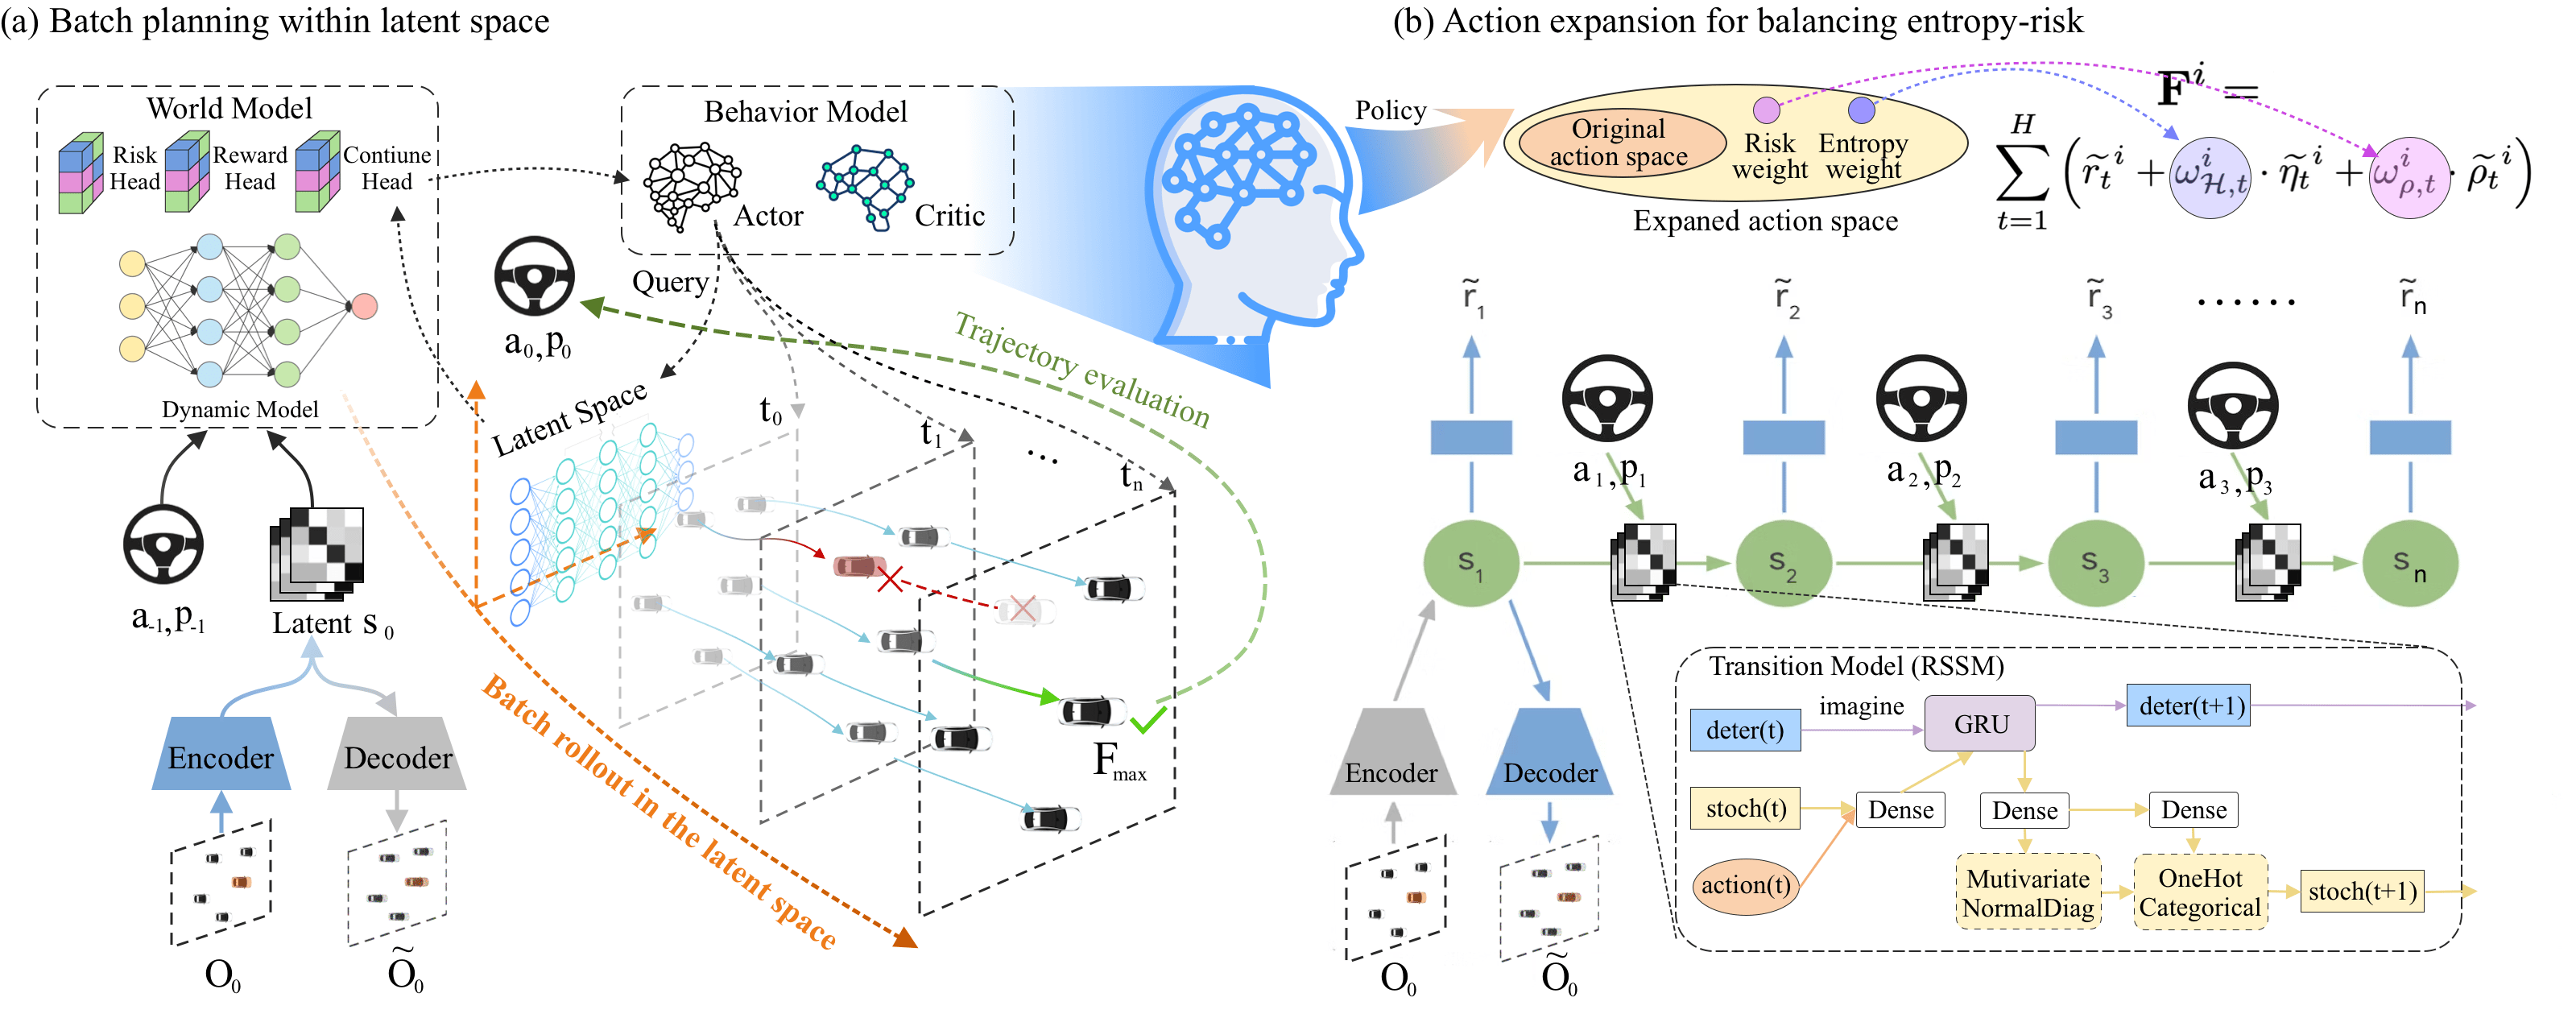
\includegraphics[width=\textwidth]{fig/Algo.png}
    \caption{Framework of the RiskDreamer algorithm. (a) Batch planning within latent space. (b) Action expansion for balancing entropy-risk. }
    \label{fig:algo}
\end{figure*}


\subsection{Planning in Latent Space}
World model\cite{ha2018world} has succeed in learning potential dynamic models capable of inferring future latent representations of the environment. The Dreamer algorithm series\cite{dreamer},\cite{dreamerv2},\cite{dreamerv3}, utilized model-based reinforcement learning through its recurrent state-space model (RSSM)\cite{RSSM}. By constructing internal world models, the algorithm enables agents to learn in virtual environments, reducing required physical interactions and enhancing both efficiency and safety in real-world applications. However, the greedy MDP behavior model in DreamerV3 struggles with long sequence decision-making, leading to suboptimal performance in continuous action sequence tasks.
Huang \textit{et al.} extended DreamerV3\cite{dreamerv3} by incorporating the Lagrangian method and Curiosity Cross-Entropy Method\cite{CCEM} to develop SafeDreamer\cite{safedreamer}. However, similar to most Lagrangian-based approaches, its performance is highly sensitive to the cost threshold \cite{gao2024enhance}. Wen \textit{et al.} \cite{CCEPETS} proposed an algorithm based on the constrained cross-entropy method, which optimizes constraints through iterative updates of elite samples. Despite its effectiveness, this approach incurs high computational costs. In contrast, our method improves planning efficiency by concurrently generating multiple imagined trajectories in latent space.
\subsection{Naturalistic Driving Simulation}
The training environment is crucial for reinforcement learning, especially in the context of autonomous driving. Current traffic simulations typically rely on either replayed data or homogenous heuristic models to emulate background traffic agents.
In a review of RL literature for autonomous vehicles, Noaeen \textit{et al.}\cite{noaeen2022reinforcement} identified that few papers incorporated simulations with diverse vehicle types. Additionally, They also noted the absence of explicit discussions about car-following parameters in autonomous vehicles RL research. Schrader \textit{et al.}\cite{sumoclibration} calibrates the parameters for each pair of car-following vehicles. However, this calibration is based on pairs of following vehicles, lacking calibration for multi-vehicle interactive movements. Yan \textit{et al.}\cite{NDE} employed neural networks to simulate the behavior of traffic agents, thereby achieving macro-level statistical realism. However, the safety mapping network mechanism they utilized does not guarantee the plausibility of microscopic traffic trajectories. 
By contrast, our method generates heterogeneous traffic agents with realistic behavior and statistics, enhancing the realism and challenge of the training environment. 



\section{Methodology}
\label{sec:method}
In this section, we present the two core concepts of the RiskDreamer framework: batch planning in the latent space and action expansion for balancing entropy and risk, as illustrated in fig. \ref{fig:algo}. Additionally, we introduce the trustworthy traffic scenario generation framework used for training and evaluating autonomous driving agents, as shown in Fig. \ref{fig:calibration}.

\subsection{Framework Overview}

The proposed RiskDreamer framework comprises three interconnected neural networks: a world model for predicting the outcomes of potential actions, a critic network for evaluating the future value of these outcomes, and a policy network for selecting actions that lead to the most valuable results. As the agent interacts with the environment, these components are trained concurrently based on replayed experiences. A central element of our approach is a batch online planner that integrates these three networks. At each decision-making step, this planner initiates a batch rollout using the world model's dynamics model. This process simultaneously explores multiple potential future trajectories within the latent space in a single rollout, offering enhanced planning efficiency. The policy network features an expanded action space, additionally outputting two balancing weights. These weights dynamically adjust the influence of expected rewards, entropy, and risk aversion at each step, derived from the world model's predictions. This transforms what are typically manually tuned hyperparameters into learnable, context-dependent strategies, enabling the agent to adapt its risk tolerance and exploration strategy according to the prevailing traffic conditions. This contrasts with other methods that rely on fixed hyperparameters, allowing for greater adaptability and potentially improved performance in complex and uncertain environments. We will now delve into the specifics of these components and their interactions.

\subsection{Preliminaries from DreamerV3}

RiskDreamer builds upon the foundation of the DreamerV3 world model. As depicted in Fig. \ref{fig:algo} (a), at each time step $t$, the world model receives an observation $\mathbf{o}_t$ and an action $\mathbf{a}_t$ as input. First, an observation encoder $\phi_{\text{enc}}$ maps the observation $\mathbf{o}_t$ to a latent representation $\mathbf{s}_t$:
\begin{equation}
\mathbf{s}_t = \phi_{\text{enc}}(\mathbf{o}_t),
\end{equation}
Given the current latent state $\mathbf{s}_t$ and action $\mathbf{a}_t$, the dynamics model $\phi_{\text{dyn}}$ predicts the next latent state $\widetilde{\mathbf{s}}_{t+1}$. The dynamics model is typically composed of a deterministic component and a stochastic component. Let $\boldsymbol{h}_t$ denote the deterministic state at time $t$. The dynamics model can be described as follows:
\begin{equation}
    \begin{split}
    \boldsymbol{h}_{t+1} &= f_{\phi}(\boldsymbol{h}_t, \mathbf{s}_t, \mathbf{a}_t), \\
    \widetilde{\mathbf{s}}_{t+1} &\sim p_{\theta}(\cdot | \boldsymbol{h}_{t+1}),
    \end{split}
\end{equation}
where $f_{\phi}$ is a deterministic function learned from $\phi_{\text{dyn}}$, and $p_{\theta}$ represents a probabilistic distribution parameterized by $\theta$. The posterior distribution of the latent state $q_{\phi}(\mathbf{s}_t | \boldsymbol{h}_t, \mathbf{o}_t)$ is inferred by combining the prior $p_{\theta}(\cdot | \boldsymbol{h}_{t})$ from the dynamics model with the current observation $\mathbf{o}_{t}$.

The world model comprises several prediction heads that decode the latent state into different modalities. In addition to the standard decoder for reconstructing the observation, and reward and continue heads from the original DreamerV3, RiskDreamer incorporates a risk prediction head. The outputs of these heads can be expressed as conditional probabilities:
\begin{equation}
    \begin{split}
    \text{Decoder}: \widetilde{\mathbf{o}}_t &\sim {\phi_{\text{dec}}}(\widetilde{\mathbf{o}}_t \mid \mathbf{s}_t), \\
    \text{RewardHead}: \widetilde{\mathbf{r}}_t &\sim {\phi_{\text{reward}}}(\widetilde{\mathbf{r}}_t \mid \mathbf{s}_t), \\
    \text{RiskHead}: \widetilde{\mathbf{\rho}}_t &\sim {\phi_{\text{risk}}}(\widetilde{\mathbf{\rho}}_t \mid \mathbf{s}_t), \\
    \text{ContinueHead}: \widetilde{\mathbf{c}}_t &\sim {\phi_{\text{cont}}}(\widetilde{\mathbf{c}}_t \mid \mathbf{s}_t),
    \end{split}
\end{equation}

where $r_t$ is the reward at time $t$, $\widetilde{\rho_t}$ is the predicted risk, and $c_t$ indicates whether the episode continues at the next step. 
The training of the world model involves minimizing a loss function that includes the reconstruction loss for each head and the KL divergence between the prior and posterior distributions of the latent states.
\begin{algorithm}[H]
    \caption{Batch Planning in Latent Space}
    \label{alg:batch_planning}
    \begin{algorithmic}[1]
    \State \textbf{Input:} Posterior distribution $\mathbf{s}_t$, embedded observation $\mathbf{e}_t$, training flag $\tau$
    \State \textbf{Parameters:} Planning horizon $H$, Batch number $N$
    \State Initialize cumulative value $\mathbb{V}$, entropy $\mathbb{E}$, and risk $\mathbb{R} \gets \mathbf{0}$
    \State Expand $\mathbf{s}_t$ to $N$ simulations: $\mathbf{s}_t \gets \text{expand}(\mathbf{s}_t, N)$
    \For{$t = 1$ to $H$}
        \If{$\tau$ and $t = 1$}  \Comment{Exploration policy}
            \State Sample actions: $\mathbf{a}_t \sim \pi_{\theta_e}(\cdot|\mathbf{s}_t)$ 
            \State Compute log probabilities: $\mathbf{L}_t \gets \log \pi_{\theta_e}(\mathbf{a}_t|\mathbf{s}_t)$
        \Else \Comment{Evaluation policy}
            \State Deterministic action: $\mathbf{a}_t \sim \pi_{\theta_t}(\cdot|\mathbf{s}_t)$ 
            \State Select actions: $\mathbf{a}_t \gets \text{mean}(\pi_{\theta_t}(\cdot|\mathbf{s}_t))$  \Comment{Use the mean of the distribution}
            \State Compute log probabilities: $\mathbf{L}_t \gets \log \pi_{\theta_t}(\mathbf{a}_t|\mathbf{s}_t)$
        \EndIf
        \State Predict next state: $\widetilde{\mathbf{s}}_{t+1} \sim \phi_{dyn}(\mathbf{s}_t, \mathbf{a}_t)$
        \State Predict risk: $\widetilde{\rho}_t \sim \phi_{risk}(\mathbf{s}_t)$
        \State Predict reward: $\widetilde{\mathbf{r}}_t \sim \phi_{rew}(\mathbf{s}_t)$
        \State Estimate policy entropy: $\widetilde{\eta_t} \gets \text{Entropy}(\pi_{\theta_e}(\cdot|\mathbf{s}_t))$
        
        \State Retrieve risk weight \(\omega_{\rho, t}\) and entropy weight \(\omega_{\mathcal{H}, t}\) from the expanded action space.
        \State \(\omega_{\mathcal{H}, t} \gets \text{action}[-1]\)  \Comment{Entropy weight}
        \State \(\omega_{\rho, t} \gets \text{action}[-2]\)  \Comment{Risk weight}
        \State Update cumulative metrics:
        \State $\mathbb{V} \gets \mathbb{V} + \widetilde{\mathbf{r}}_t$, $\mathbb{E} \gets \mathbb{E}$ + $\omega_{\mathcal{H}, t}$ $\cdot$  $\widetilde{\eta_t}$, $\mathbb{R} \gets \mathbb{R} + \omega_{\rho, t} \cdot \widetilde{\rho_t}$
        \State Store actions: $\mathbf{A}_t \gets \mathbf{a}_t$
        \State Update state: $\mathbf{s}_t \gets \mathbf{s}_{t+1}$
    \EndFor
    \State Compute objective: $\mathbf{F} \gets \mathbb{V} + \mathbb{E} + \mathbb{R}$
    \State Select best simulation: $i^* \gets \arg\max(\mathbf{F})$
    \State \textbf{Output:} Best action $\mathbf{a}_{i^*}$, log probability $\mathbf{L}_{i^*}$
    \end{algorithmic}
\end{algorithm}
% The training of the world model involves minimizing a loss function that includes the reconstruction loss for each head and the KL divergence between the prior and posterior distributions of the latent states. The loss function can be expressed as:

% \begin{equation}
%     \begin{split}
%     \mathcal{L}_{WM} = \mathbb{E}_{p_{data}} \Big[
%     & -\log p_{\phi_{\text{dec}}}(\mathbf{o}_t | \mathbf{s}_t)
%     - \log p_{\phi_{\text{reward}}}(r_t | \mathbf{s}_t) \\
%     & - \log p_{\phi_{\text{risk}}}(\rho_t | \mathbf{s}_t)
%     - \log p_{\phi_{\text{cont}}}(c_t | \mathbf{s}_t) \\
%     & + D_{KL}(\underbrace{q_{\phi}(\mathbf{s}_t | \mathbf{s}_{t-1}, \mathbf{a}_{t-1}, \mathbf{o}_t)}_{\text{Posterior}} \\
%     & || \ \underbrace{p_{\theta}(\mathbf{s}_t | \mathbf{s}_{t-1}, \mathbf{a}_{t-1})}_{\text{Prior}})
%     \Big],
%     \end{split}
% \end{equation}
% The KL divergence term encourages the prior distribution of the latent state $\mathbf{s}_t$ predicted by the dynamics model, $p_{\theta}$, to be close to the posterior distribution, $q_{\phi}$, inferred after observing $\mathbf{o}_t$.

% debug
% The expectation $\mathbb{E}_{p_{data}}$ is taken over trajectories from the replay buffer, consisting of observations ($\mathbf{o}_{1:T}$), actions ($\mathbf{a}_{1:T}$), rewards ($r_{1:T}$), risks ($\rho_{1:T}$), and continue flags ($c_{1:T}$).  The first four terms encourage the world model to accurately reconstruct the observations and predict the reward, risk, and continue signals based on the latent state $\mathbf{s}_t$.

% The final term is the KL divergence, weighted by a factor $\beta$, between the posterior distribution $q_{\phi}(\mathbf{s}_t | \mathbf{h}_{t}, \mathbf{o}_t)$ and the prior distribution $p_{\theta}(\mathbf{s}_t | \mathbf{h}_{t})$.  The posterior, also known as the *representation model* in Dreamer, infers the latent state $\mathbf{s}_t$ given the deterministic state $\mathbf{h}_t$ and the current observation $\mathbf{o}_t$. The prior, part of the *transition model*, predicts the latent state $\mathbf{s}_t$ given only the deterministic state $\mathbf{h}_t$ (which is computed from the previous latent state $\mathbf{s}_{t-1}$ and action $\mathbf{a}_{t-1}$).  Minimizing the KL divergence encourages the transition model to predict latent states that are consistent with those inferred from the observations, thus learning a reliable dynamics model. The weight $\beta$ balances the reconstruction accuracy and the latent dynamics regularization. Following DreamerV3, we use a free bits implementation by clipping the KL divergence term from below to avoid vanishing KL term gradients:

% \begin{equation}
%     \begin{split}
%          D_{KL}(q||p) = max(D_{KL}(q||p), \lambda)
%     \end{split}
% \end{equation}
% Where \(\lambda\) is a hyperparameter.

% The deterministic state $\mathbf{h}_t$ is updated using a recurrent neural network (RNN), typically a Gated Recurrent Unit (GRU), within the dynamics model $\phi_{\text{dyn}}$:
% \begin{equation}
% \mathbf{h}_t = f_{\phi}(\mathbf{h}_{t-1}, \mathbf{s}_{t-1}, \mathbf{a}_{t-1}).
% \end{equation}

% Both the posterior $q_{\phi}$ and prior $p_{\theta}$ are modeled as Gaussian distributions with diagonal covariance matrices. The parameters of these distributions are predicted by neural networks.
%debug

% \begin{equation}
%     \begin{split}
%     \mathcal{L}_{WM} = \mathbb{E}_{(\mathbf{o}, \mathbf{a}, r, \rho, c) \sim \mathcal{D}} \Big[
%      & -\log p_{\phi_{\text{dec}}}(\mathbf{o}_t | \mathbf{s}_t) 
%      -\log p_{\phi_{\text{reward}}}(r_t | \mathbf{s}_t) \\
%     & -\log p_{\phi_{\text{risk}}}(\rho_t | \mathbf{s}_t) 
%     -\log p_{\phi_{\text{cont}}}(c_t | \mathbf{s}_t)  \\
%     & + \beta \cdot \max\left(D_{KL}(q_{\phi}(\mathbf{s}_t | \mathbf{h}_{t}, \mathbf{o}_t) \\
%     || p_{\theta}(\mathbf{s}_t | \mathbf{h}_{t})), \lambda\right)  \Big],
%     \end{split}
%     \label{eq:world_model_loss}
% \end{equation}

\begin{equation}
    \begin{split}
    \mathcal{L}_{WM} = \mathbb{E}_{(\mathbf{o}, \mathbf{a}, r, \rho, c) \sim \mathcal{D}} \Big[
    &-\log p_{\phi_{\text{dec}}}(\mathbf{o}_t | \mathbf{s}_t) 
    -\log p_{\phi_{\text{reward}}}(r_t | \mathbf{s}_t) \\
    &-\log p_{\phi_{\text{risk}}}(\rho_t | \mathbf{s}_t) 
    -\log p_{\phi_{\text{cont}}}(c_t | \mathbf{s}_t)  \\
    &+ \beta \cdot \max \Big( D_{KL} \big( q_{\phi}(\mathbf{s}_t | \mathbf{h}_{t}, \mathbf{o}_t) \\
    &  \big\| p_{\theta}(\mathbf{s}_t | \mathbf{h}_{t}) \big), \lambda \Big) \Big],
    \end{split}
    \label{eq:world_model_loss}
    \end{equation}
    The expectation $\mathbb{E}$ is over trajectories from the replay buffer $\mathcal{D}$, which includes observations $\mathbf{o}$, actions $\mathbf{a}$, rewards $r$, risks $\rho$, and continue flags $c$. The loss function promotes accurate reconstruction of observations and prediction of rewards, risks, and continue flags, conditioned on the latent state $\mathbf{s}_t$.

    A KL divergence term, scaled by $\beta$, regularizes the latent dynamics.  This term minimizes the difference between the posterior distribution $q_{\phi}(\mathbf{s}_t | \mathbf{h}_{t}, \mathbf{o}_t)$ (representation model) and the prior distribution $p_{\theta}(\mathbf{s}_t | \mathbf{h}_{t})$ (transition model).  The posterior infers $\mathbf{s}_t$ from the deterministic state $\mathbf{h}_t$ and observation $\mathbf{o}_t$, while the prior predicts $\mathbf{s}_t$ solely from $\mathbf{h}_t$.  This regularization ensures consistency between the transition model's predictions and the observations.  The $\max$ function, with threshold $\lambda$, implements the "free bits" method to prevent vanishing KL gradients.
    
    The deterministic state $\mathbf{h}_t$ is updated recurrently via the dynamics model $\phi_{\text{dyn}}$, typically using a GRU:
    
    \begin{equation}
    \mathbf{h}_t = f_{\phi}(\mathbf{h}_{t-1}, \mathbf{s}_{t-1}, \mathbf{a}_{t-1}).
    \end{equation}
    
    Both $q_{\phi}$ and $p_{\theta}$ are modeled as diagonal Gaussian distributions, with parameters determined by neural networks.

The actor-critic component in RiskDreamer, similar to classic SAC \cite{SAC}, consists of an actor network $\pi_{\theta}(\mathbf{a}_t | \mathbf{s}_t)$ and a value network $V_{\psi}(\mathbf{s}_t)$. The actor network predicts a distribution over actions, while the value network estimates the expected future reward.

\subsection{Batch Planning within Latent Space}
The batch planning method of RiskDreamer leverages the world model to efficiently explore potential future scenarios. Instead of serially simulating one trajectory at a time, it generates and evaluates multiple trajectories in parallel within the latent space. The process begins with the current latent state $\mathbf{s}_t$ and the embedded observation $\mathbf{e}_t = \phi_{\text{enc}}(\mathbf{o}_t)$. 

The batch planning process can be summarized in Algorithm \ref{alg:batch_planning}. The algorithm takes as input the current latent state $\mathbf{s}_t$, the embedded observation $\mathbf{e}_t$, and a training flag $\tau$ that determines whether the exploration policy or the evaluation policy is used. The algorithm also requires the planning horizon $H$ and the number of simulations $N$ to be specified. The latent state $\mathbf{s}_t$ is expanded to $N$ simulations, each of which is used to simulate a potential trajectory.



At each planning step within the horizon, the policy network proposes actions for each of the $N$ simulated trajectories. For training ($\tau$ is true) and in the first step ($t=1$), an exploration policy $\pi_{\theta_e}$ is used to sample actions, encouraging policy diversity. Subsequently, or during evaluation ($\tau$ is false or $t>1$), the evaluation policy $\pi_{\theta_t}$ is employed, and the action with the highest probability is selected. The world model then predicts the subsequent latent state for each simulation based on the chosen action. At each step $t$ of the planning horizon, the algorithm also predicts the risk $\widetilde{\rho_t}$ and the value $\widetilde{v_t}$ of the current state, and estimates the entropy $\widetilde{\eta_t}$ of the policy.

The value of each imagined trajectory is implicitly evaluated through the cumulative sum of the predicted values, estimated policy entropies, and predicted risks. Let the $N$ simulations be indexed. The cumulative value $\mathbb{V}$, entropy $\mathbb{E}$, and risk $\mathbb{R}$ are updated at each step $t$ for each simulation. Specifically, for each simulation $i \in \{1, \dots, N\}$:

\begin{equation}
    \begin{split}
        \mathbb{V}^i &\gets \mathbb{V}^i + \widetilde{v_t}^i, \\
        \mathbb{E}^i &\gets \mathbb{E}^i + \omega_{\mathcal{H}, t}^i \cdot \widetilde{\eta_t}^i, \\
        \mathbb{R}^i &\gets \mathbb{R}^i + \omega_{\rho, t}^i \cdot \widetilde{\rho_t}^i,
    \end{split}
\end{equation}


The objective $\mathbf{F}$ for each simulation is calculated as the sum of the cumulative value, entropy, and risk at the end of the planning horizon $H$:
\begin{equation}
    \mathbf{F}^i = \mathbb{V}^i + \mathbb{E}^i + \mathbb{R}^i = \sum_{t=1}^{H} \left( \widetilde{r_t}^i + \omega_{\mathcal{H}, t}^i \cdot \widetilde{\eta_t}^i + \omega_{\rho, t}^i \cdot \widetilde{\rho_t}^i \right),
\end{equation}

Finally, the simulation with the highest objective is selected, and the first action of that simulation is returned as the best action. This batch planning approach allows the agent to consider a set of potential future scenarios in parallel and make decisions based on the aggregated value, entropy, and risk.

\subsection{Action Expansion for Balancing Entropy and Risk}
A key innovation of RiskDreamer is the expansion of the policy network's action space. Instead of directly outputting only the action to be taken in the environment, the policy network in RiskDreamer outputs additional parameters that control the balance between exploration, exploitation, and risk aversion. Specifically, the action output by the policy network $\pi_{\varphi}$ is augmented to include weights for entropy and risk:
\begin{equation}
\mathbf{a}_t = [\mathbf{a}^{\prime}_{t}, \omega_{\rho, t}, \omega_{\mathcal{H}, t}],
\end{equation}
where $\mathbf{a}^{\prime}_{t}$ represents the action to be executed in the environment, $\omega_{\rho, t} \in [-1, 1]$ is the weight assigned to the predicted risk, and $\omega_{\mathcal{H}, t} \in [-1, 1]$ is the weight assigned to the entropy of the state and policy distributions.

These weights are outputs of the policy network and are conditioned on the current latent state $\mathbf{s}_t$:
\begin{equation}
    \begin{split}
        \omega_{\rho, t} &= \pi_{\varphi}^{\rho}(\mathbf{s}_t), \\
        \omega_{\mathcal{H}, t} &= \pi_{\varphi}^{\mathcal{H}}(\mathbf{s}_t).
    \end{split}
\end{equation}
During the batch planning process, these weights are used to modulate the contribution of risk and entropy to the evaluation of each imagined trajectory. By making these balancing factors outputs of the policy network, RiskDreamer enables the agent to dynamically adapt its risk tolerance and exploration strategy based on the specific context and perceived risk of the situation. For instance, in high-risk scenarios, the policy network might learn to increase $\omega_{\rho}$ to prioritize risk aversion, while in less critical situations, it might increase $\omega_{\mathcal{H}}$ to encourage exploration. This mechanism provides a more flexible and adaptive approach compared to using fixed hyperparameters for balancing these factors.




% #####################################

    % needed in second column of first page if using \IEEEpubid
    %\IEEEpubidadjcol
\begin{figure*}[htbp]
    \centering
    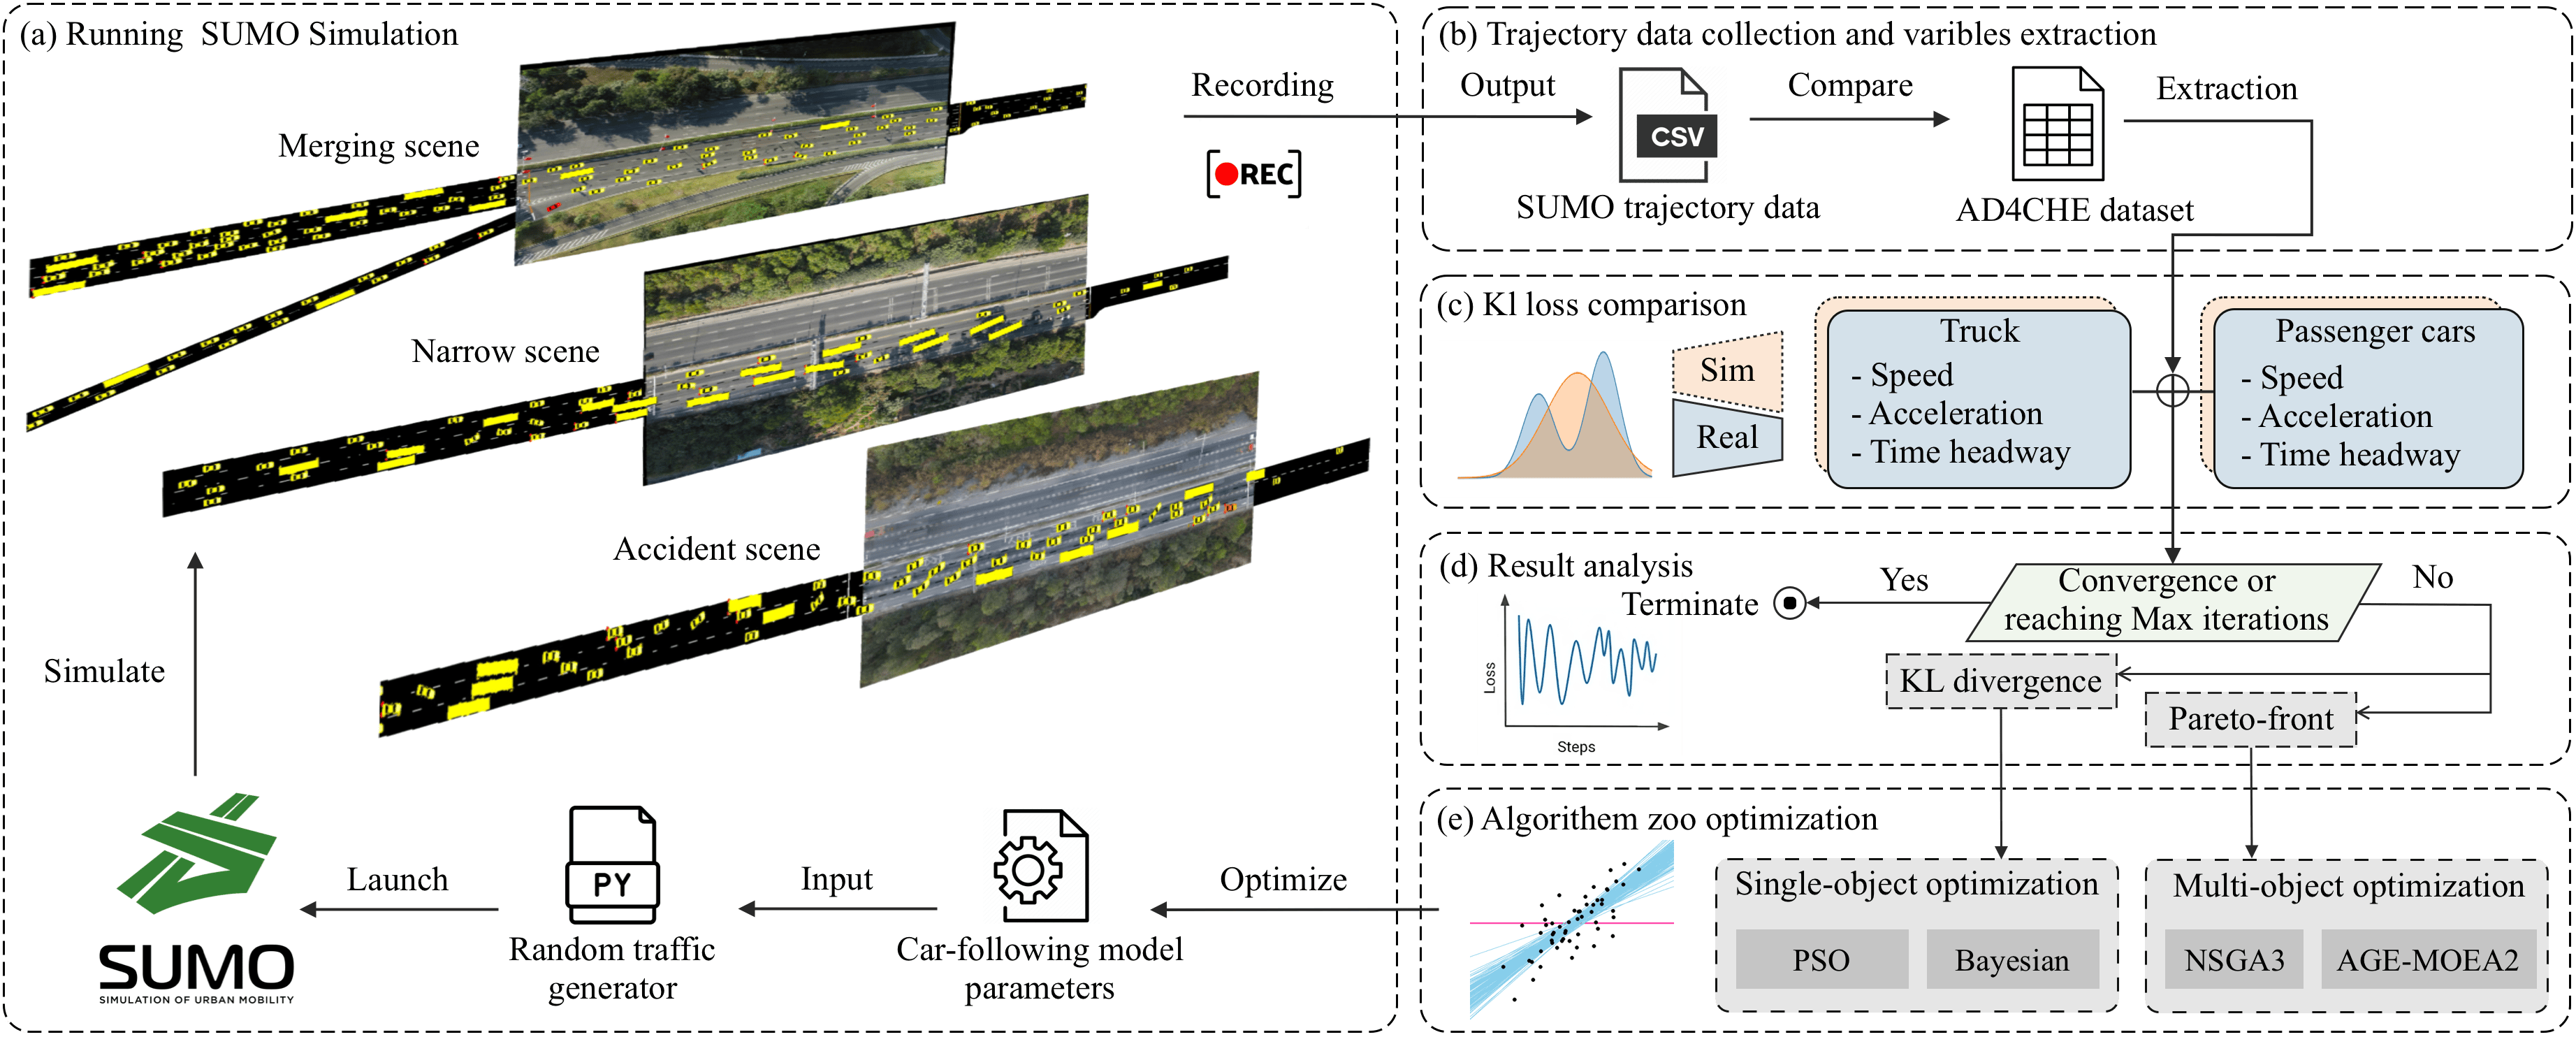
\includegraphics[width=\textwidth]{fig/calibration_framework.png}
    \caption{Calibration framework of the trustworthy traffic simulation}
    \label{fig:calibration}
\end{figure*}

\subsection{Trustworthy Traffic Scenario Generation}
To make simulation an effective tool for developing autonomous driving algorithms, the simulator needs to generate realistic traffic scenarios with precise distributions that accurately reflect the behavior of background traffic agents.

We achieve this by calibrating the parameters of EIDM \cite{EIDM} car-following models using aggregated feature distributions derived from real-world vehicle trajectory datasets as optimization targets.
Through iterative refinement of these parameter distributions, we minimize the divergence between simulated and real trajectory features, thereby generating realistic and naturally interactive driving behaviors for background traffic agents.

Fig. \ref{fig:calibration} illustrates our generation process in detail. In step (a), we run the simulator as a black-box, high-cost function in the optimization process. Specifically, the simulator can be represented as a function $f(\mathbf{x})$, where $\mathbf{x} = [x_1, x_2, \ldots, x_N]^\top$ is the vector of input parameters for the car-following model that drives the background traffic agents. These parameters are subject to the inequality constraints specified by the boundaries shown in Table \ref{tab:parameter_bounds}:


\begin{table}[ht]
\centering
\caption{Boundaries of the car-following model parameters}
\label{tab:parameter_bounds}
\begin{tabular}{p{1.2cm}p{4.5cm}p{0.9cm}p{0.9cm}}
\toprule
\multicolumn{1}{c}{\textbf{Parameters}} & \multicolumn{1}{c}{\textbf{Descriptions (Unit)}} & \multicolumn{1}{c}{\textbf{Car}} & \multicolumn{1}{c}{\textbf{Bus}} \\
\midrule                 
$\tau_{\text{mean}}$ & Average time headway (\si{\second}) & (0.5, 4) & (0.5, 4) \\
$\tau_{\text{std}}$ & Std. deviation of time headway ($-$)  & (0, 10) & (0, 10) \\
$v_{\text{mean}}$ & Average max speed (\si{\meter/\second}) & (8, 26) & (8, 26) \\
$v_{\text{std}}$ & Std. deviation of max speed ($-$) & (0, 20) & (0, 20) \\
$a$ & Max acceleration (\si{\meter/\second^{2}}) & (0.2, 4)  & (0.2, 4) \\
$d$ & Max deceleration  (\si{\meter/\second^{2}}) & (0.2, 4) & (0.2, 4) \\
$L_{\text{sublane}}$ & Eagerness to align laterally in-lane ($-$) & (0, 1) & (0, 1) \\
$L_{\text{pushy}}$ & Willingness to encroach laterally ($-$) & (0, 1) & (0, 1) \\
$L_{\text{speed\_gain}}$ & Lane-changing for speed gain ($-$) & (0, 5) & (0, 5) \\
$L_{\text{assertive}}$ & Acceptance of smaller gaps ($-$) & (1, 100) & (1, 100) \\
$L_{\text{cooperative}}$ & Cooperative lane-changing ($-$) & (0, 1) & (0, 1) \\
$L_{\text{lookahead}}$ & Adjustment for lookahead distance (\si{\meter}) & (2, 100) & (2, 100) \\
\bottomrule
\end{tabular}
\end{table}

Meanwhile, the scenario configurations, including road topology, traffic flow, and vehicle type distribution, are pre-established based on the statistical properties of the dataset.

The trajectory data generated by the simulator will undergo (b) trajectory data collection and variable extraction. This process yields aggregated distributions of variables such as speed, acceleration, and headway for different types of agents (e.g., trucks and passenger cars). Subsequently, we employ the Kullback-Leibler (KL) divergence to compare the aggregated feature distributions between the simulated and real-world data. The KL divergence for the $m$-th feature is calculated as:

\begin{equation}
D_{\mathrm{KL}}^{(m)} = \sum_{i} p_i^{(m)} \log \left( \frac{p_i^{(m)}}{q_i^{(m)}} \right),
\end{equation}

where $p_i^{(m)}$ and $q_i^{(m)}$ are the probability distributions of the $m$-th feature from the simulated data and the real data, respectively. The set of KL divergences $\{ D_{\mathrm{KL}}^{(1)}, D_{\mathrm{KL}}^{(2)}, \ldots, D_{\mathrm{KL}}^{(M)} \}$ serve as the objectives in the optimization task.

Our goal is to solve the following optimization problem:

\begin{equation}
\begin{aligned}
\min_{\mathbf{x}} \quad & \mathbf{F}(\mathbf{x}) = [D_{\mathrm{KL}}^{(1)}, D_{\mathrm{KL}}^{(2)}, \ldots, D_{\mathrm{KL}}^{(M)}], \\
\text{s.t.} \quad & x_i^{L} \leq x_i \leq x_i^{U}, \quad i = 1, \ldots, N.
\end{aligned}
\end{equation}
where $x_i^{L}$ and $x_i^{U}$ are the lower and upper bounds for the $i$-th parameter.
In step (d), result analysis, we compare the optimization outcomes with our predefined convergence criteria to determine whether to continue optimization iterations. When using multi-objective optimization, we can manually adjust the weights of each optimization objective or examine the Pareto front to understand the trade-offs between different objectives.

We utilize (e) state-of-the-art algorithms from\cite{bsy}\cite{pymoo} to optimize a new set of parameters for running the simulations.







\begin{figure*}[htbp]
    \centering
    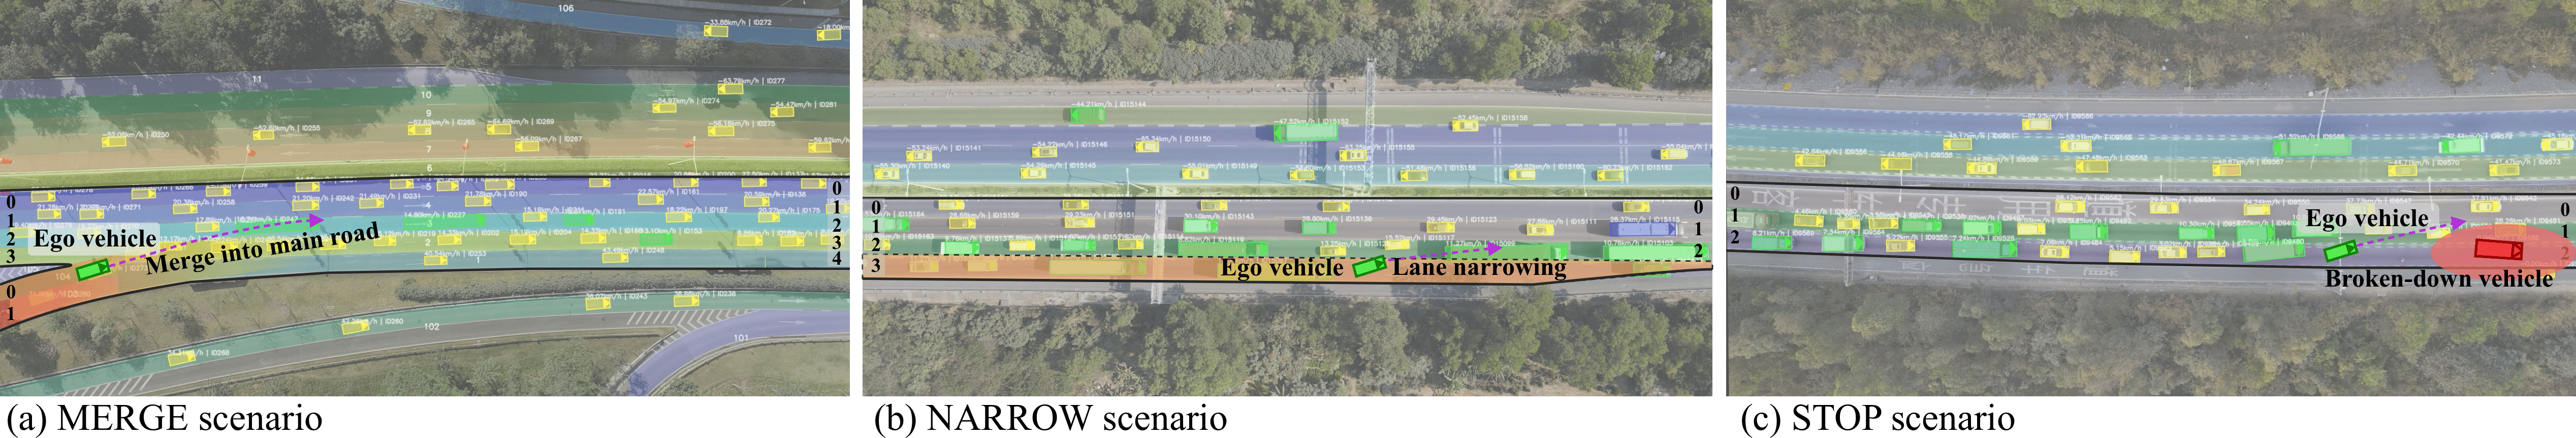
\includegraphics[width=\textwidth]{fig/sim.png}
    \caption{Three scenarios in the simulation environment: (a) MERGE: vehicle merging into the main lane from the ramp, (b) NARROW: vehicle navigating a narrowing right lane, (c) STOP: vehicle bypassing a broken-down vehicle.}
    \label{fig:sim}
\end{figure*}
\begin{figure*}[!htbp]
    \centering
    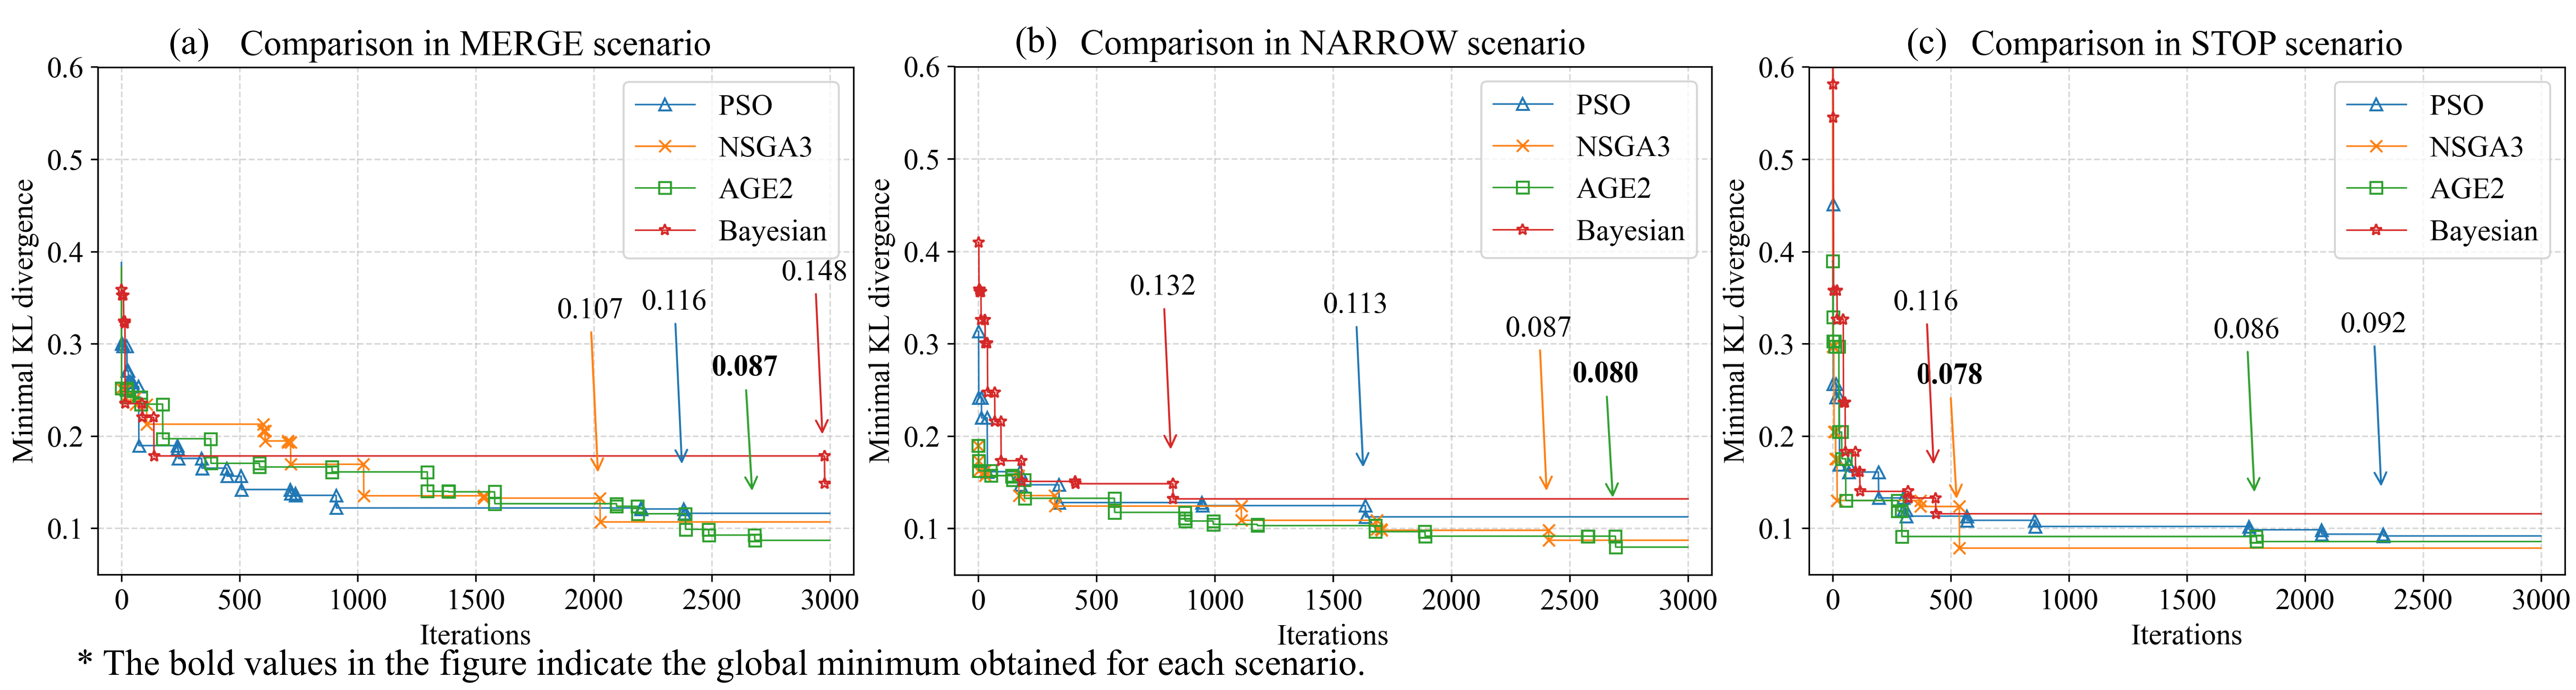
\includegraphics[width=\textwidth]{fig/env_iter.png}
    \caption{
        Convergence comparison of optimization objective in (a) MERGE scenario, (b) NARROW scenario, (c) STOP scenario. 
    }
    \label{fig:env_iter}
\end{figure*}

\begin{figure*}[!htbp]
    \centering
    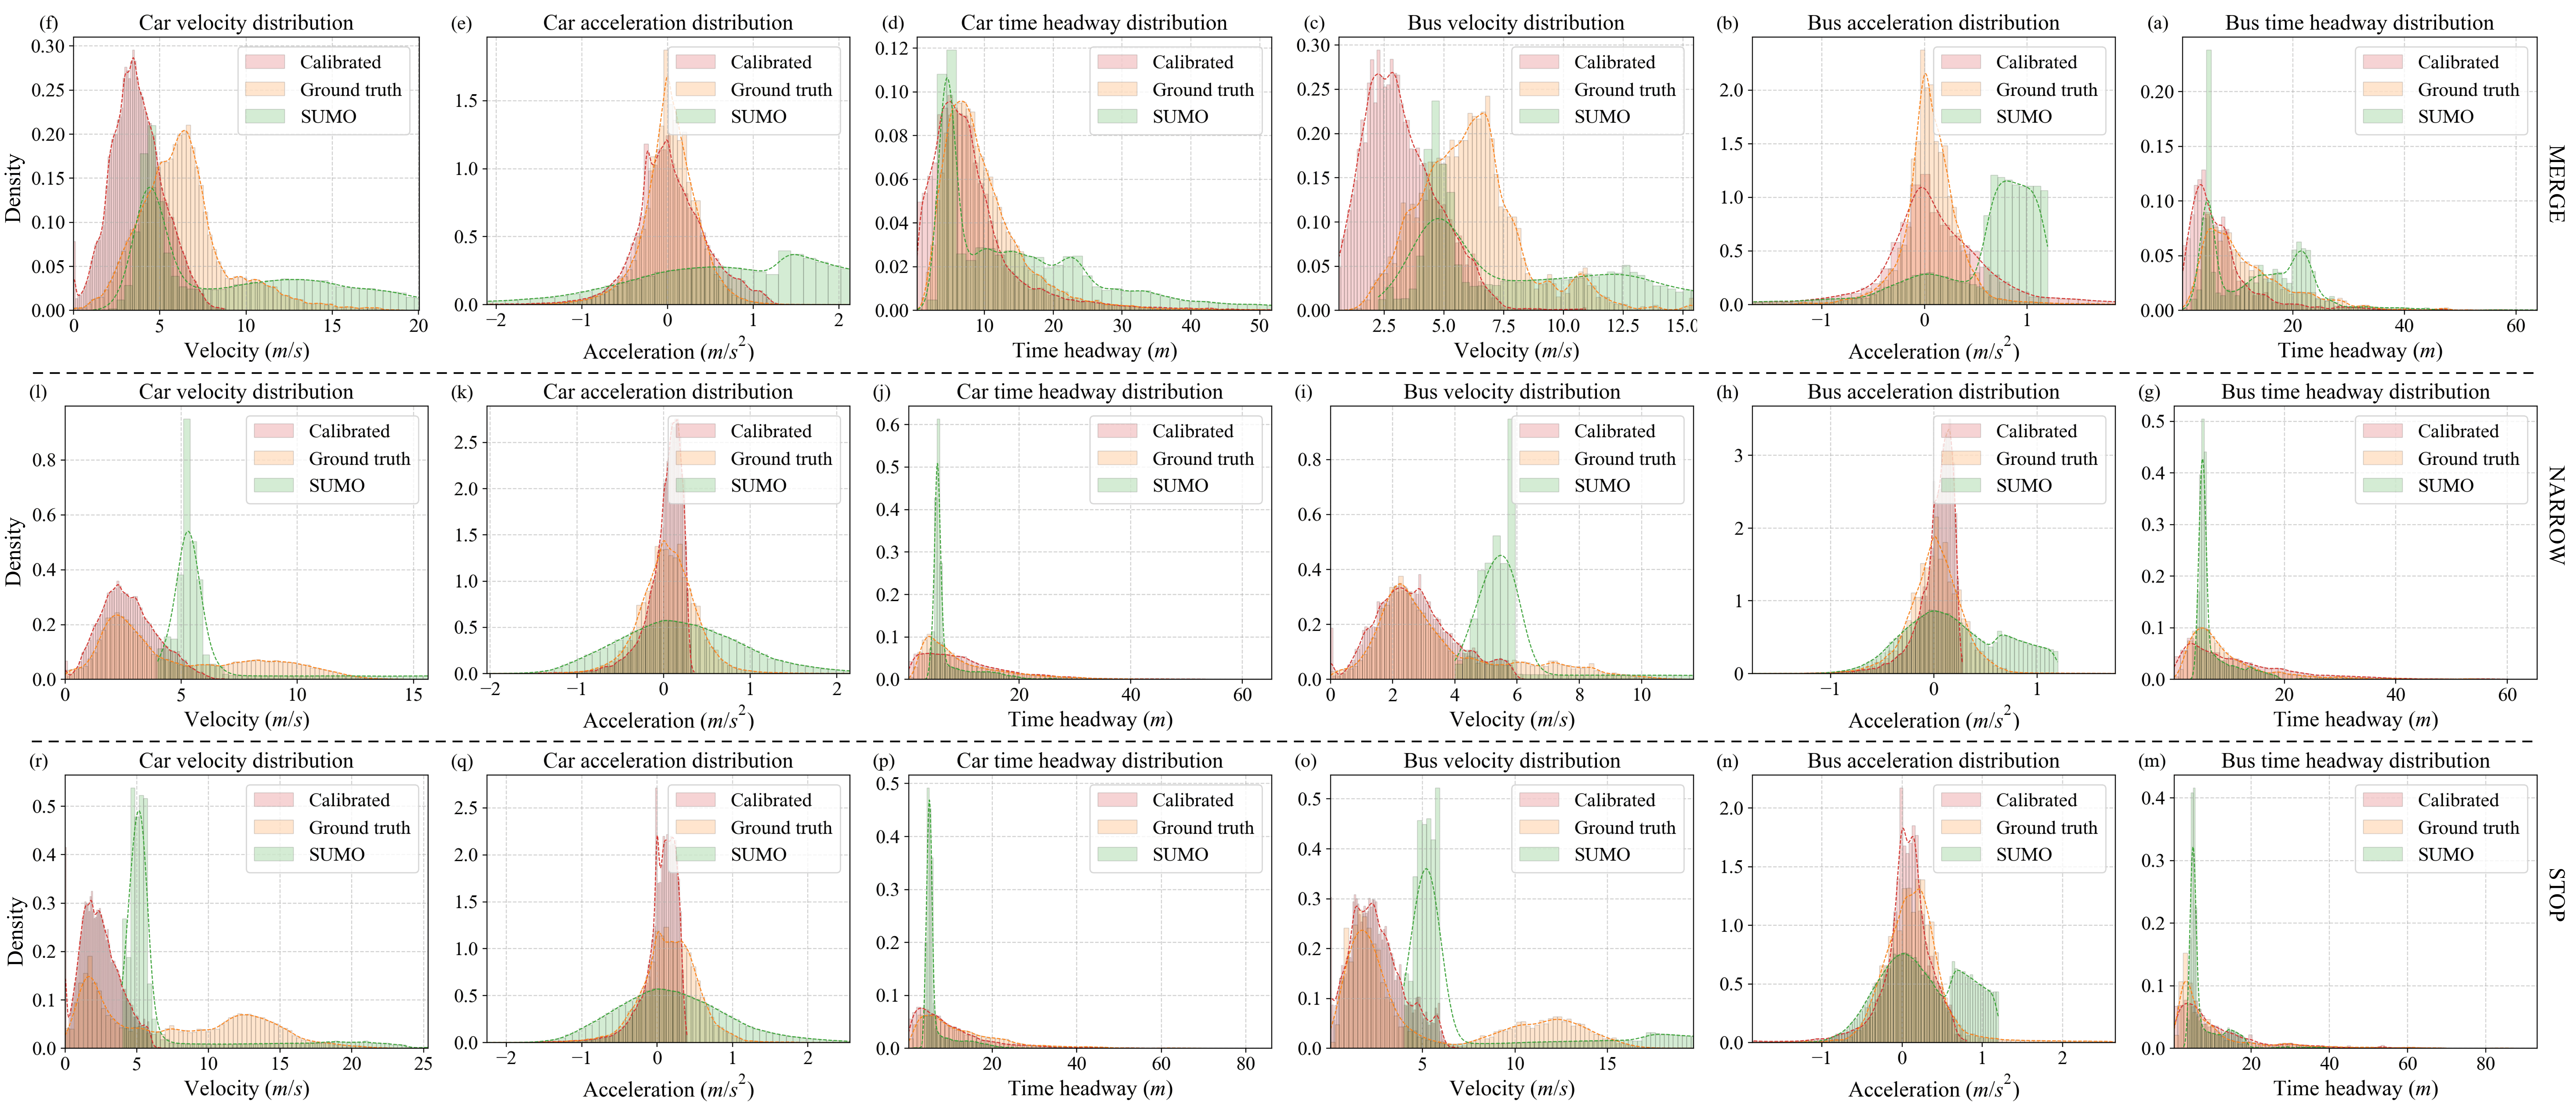
\includegraphics[width=\textwidth]{fig/env_dis.png}
    \caption{Comparison of calibration results for velocity, acceleration, and time headway distributions across three scenarios for cars and buses}
    \label{fig:env_distri}
\end{figure*}


\section{Experiments and Results}
\label{sec:experiments}
% I. Broad Context and Significance (Setting the Stage):
% A Opening Hook
This section details the experimental evaluation conducted to validate the performance of our proposed algorithm within realistic simulated traffic scenarios. We trained and evaluated our algorithm against seven baselines, followed by a comprehensive analysis of the experimental results, including an ablation study. The subsequent subsections elaborate on the experimental setup, traffic scenario generation, training procedures, and results analysis.

\subsection{Simulation Environment}
Adversarial congestion scenarios, including mandatory lane changes during merges, accidents, and lane narrowing, pose critical challenges to highway automation. These scenarios are major contributors to autonomous driving system failures \cite{naturecrash, nordhoff2024conceptual}. To evaluate our method's performance under such conditions, we utilized the AD4CHE dataset \cite{AD4CHE}, which focuses on congestion on Chinese highways and urban highways.

We selected three representative scenarios from AD4CHE's aerial data (5.12 hours total): (a) Merge scenario (files 1-8), where the ego vehicle merges from a two-lane road onto a four-lane highway, requiring conflict resolution in the merging zone; (b) Narrow scenario (files 18-23), where the ego vehicle must change lanes leftward before a road narrowing; and (c) Stop scenario (files 15-16), where the ego vehicle navigates around a broken-down vehicle in slow-moving traffic.  These scenarios are illustrated in Fig. \ref{fig:sim}.

\subsection{Trustworthy Traffic Scenario Generation}

We utilize SUMO\cite{SUMO2018} (Simulation of Urban MObility) to create the simulation environment. Four optimization algorithms—PSO\cite{pso}, Bayesian\cite{bayesian}, NSGA3\cite{NSGA3}, and AGE2\cite{AGE2}—are employed to minimize the KL divergence between the aggregated real-world and simulated data for acceleration, velocity, and time headway. Each algorithm iterates 3000 times (population-based and evolutionary algorithms use 100 populations$\times$30 iterations to ensure fair results.)

The calibrated aggregated traffic flow metrics include acceleration, velocity, and time headway distributions for both car and bus vehicle types. These calibration results are compared against both the real-world dataset and the original SUMO-generated metrics. The calibration process was done in a workstation equipped with 2$\times$AMD 5995WX CPU (128 cores total) and 256GB of RAM, required approximately 24 hours to complete 3000 iterations across three scenarios for four algorithms.

Fig. \ref{fig:env_iter} shows the convergence comparison of the optimization objective in the three scenarios. The results show that all four optimization algorithms can reduce the error to a satisfactory level (mean KL divergence around 0.1). Single-objective algorithms (PSO, Bayesian) typically converge to the minimum value more quickly, while multi-objective algorithms (NSGA3, AGE2) ultimately achieve smaller values within a limited number of iterations. 

Fig. \ref{fig:env_distri} presents the distributions of multiple calibrated traffic flow aggregation metrics, compared with both the real dataset and uncalibrated original SUMO-generated metrics. The results demonstrate that, except for a few scenarios shown in Fig. \ref{fig:env_distri} (c) and (f), the calibrated metric distributions generally align with the true dataset in terms of central tendency, while the original SUMO-generated distributions typically exhibit wider dispersion. The time headway distributions in both real and calibrated data reveal a characteristic skewed pattern with peaks at smaller time intervals, indicating the presence of aggressive driving behaviors in the dataset. The original SUMO distributions shows significant deviations at larger time headways ($\ge$\SI{10}{\meter}), particularly underestimating the frequency of large time headways in complex scenarios such as MERGE and NARROW.
Regarding acceleration, the calibrated distributions show a more pronounced peak near zero acceleration, closely matching the ground truth distribution, while the SUMO distribution exhibits a shifted peak.  In the STOP scenario, SUMO severely underestimates the frequency of negative accelerations, whereas the calibrated model more accurately reflects actual braking behavior. Finally, the calibrated speed distributions effectively capture the bimodal characteristics (a high-frequency region and a more dispersed long-tail distribution), significantly outperforming SUMO. This improvement is particularly evident in the MERGE and STOP scenarios for cars, where SUMO notably overestimates speeds in the mid-range (e.g., \SIrange{5}{10}{\metre\per\second}) and underestimates the long-tail low-speed region. The calibrated model demonstrably corrects these deficiencies.





\subsection{Agent Training and Evaluation Setup}
To ensure experimental reproducibility, all agents were trained across five random seeds, each for 1000 episodes. Each episode was limited to 3000 time steps. Both training and evaluation were performed in trustworthy traffic scenarios, as described earlier in this paper. 
The experiments were conducted on a workstation equipped with dual NVIDIA RTX 3090 GPUs, an AMD Ryzen 9950X CPU, and 64 GB of RAM. The training process took approximately 12 hours. The following sections provide detailed information on the agent configuration.

\begin{figure}[H]
    \centering
    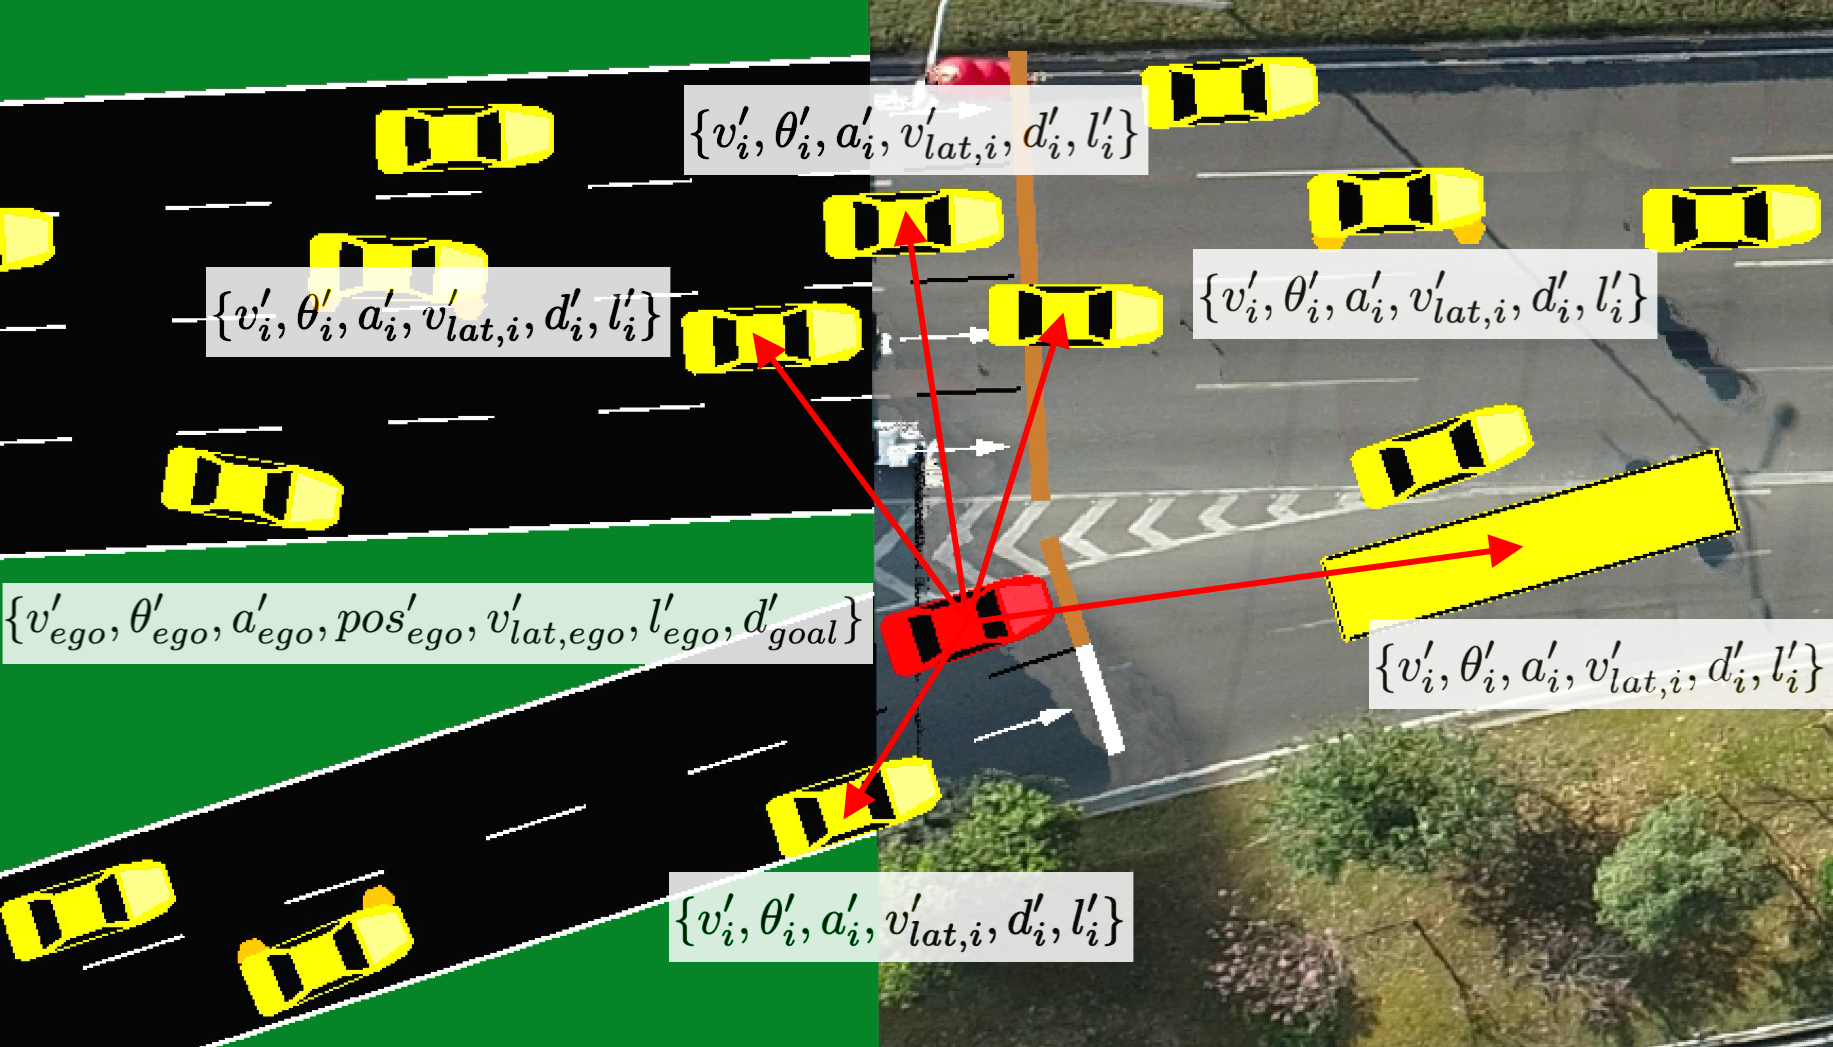
\includegraphics[width=0.49\textwidth]{fig/sim_set_up.png}
    \caption{Observation space for ego agent}
    \label{fig:sim_set_up} 
\end{figure}




\textbf{Observation Space:}
The observation space $\mathbf{o}_{t}$ is updated at \SI{10}{\hertz} and provides the agent's perception of its surroundings. It is formed by concatenating the observation vectors of the five nearest vehicles within a \SI{100}{\meter} detection range, together with the ego vehicle's own state as shown in Fig. \ref{fig:sim_set_up}. The observation space is defined as:
\begin{equation}
    \mathbf{o}_{t} = [\mathbf{o}_{\text{veh},i}]_{i=1, \ldots, 5} \oplus \mathbf{o}_{\text{ego}}.
\end{equation}

For each of the five nearest vehicles ($i = 1, 2, \ldots, 5$), the observation vector is a 6-dimensional set of normalized parameters:
\begin{equation}
    \mathbf{o}_{\text{veh},i} = \{v'_{\text{i}}, \theta'_{\text{i}}, a'_{\text{i}}, v'_{\text{lat},i}, d'_{\text{i}}, l'_{\text{i}}\},
\end{equation}
where $v'_{\text{i}}$, $\theta'_{\text{i}}$, $a'_{\text{i}}$, $v'_{\text{lat},i}$, $d'_{\text{i}}$, and $l'_{\text{i}}$ respectively represent the $i$-th vehicle's normalized speed, angle, acceleration, lateral speed, distance, and length.

The ego vehicle's observation vector consists of seven dimensions:
\begin{equation}
    \mathbf{o}_{\text{ego}} = \{v'_{\text{ego}}, \theta'_{\text{ego}}, a'_{\text{ego}}, pos'_{\text{ego}}, v'_{\text{lat,ego}}, l'_{\text{ego}}, d'_{\text{goal}}\},
\end{equation}
incorporating the ego vehicle's normalized speed, angle, acceleration, lane position, lateral speed, length, and distance to goal.

Table~\ref{tab:obs} summarizes each variable in the observation space:

\begin{table}[!ht]
    \centering
    \caption{Observation variables and their normalization.}
    \label{tab:obs}
    \begin{tabularx}{\columnwidth}{cX} % 使用 cX,第一列居中,第二列 X 列默认居中
    \toprule
    \textbf{Symbol} & \textbf{Description and Normalization} \\
    \midrule
    $v'_{\text{i}}, v'_{\text{ego}}$           & Vehicle speed, normalized by $v_{\text{max}}$ \\
    $\theta'_{\text{i}}, \theta'_{\text{ego}}$ & Vehicle angle, normalized by $\theta_{\text{max}}$ \\
    $a'_{\text{i}}, a'_{\text{ego}}$           & Vehicle acceleration, normalized by $a_{\text{max}}$ \\
    $v'_{\text{lat},i}, v'_{\text{lat,ego}}$   & Lateral speed, normalized by $v_{\text{lat,max}}$ \\
    $d'_{\text{i}}$                     & Distance to the $i$-th vehicle, normalized by $d_{\text{detect}}$ \\
    $l'_{\text{i}}, l'_{\text{ego}}$           & Vehicle length, normalized by $l_{\text{norm}}$ \\
    $pos'_{\text{ego}}$                 & Ego lane position, normalized by $d_{lane}$ \\
    $d'_{\text{goal}}$                  & Distance to goal, normalized by $d_{goal,init}$  \\
    \bottomrule
    \end{tabularx}
\end{table}

\textbf{Action Space:}
The action space $\mathbf{a}_t$ is a two-dimensional vector:
\begin{equation}
    \mathbf{a}_t = \{a_t, \delta_t\},
\end{equation}
where $a_t$ represents the acceleration and $\delta_t$ the lateral movement. Both components are continuous values within the range $[-1, 1]$. When interacting with the simulator, the acceleration $a_t$ is scaled by $a_{\text{max}}$, while $\delta_t$ remains unchanged as defined by the SUMO interface.


% =========debug=========
\textbf{Reward Function:}
The reward $\mathrm{R}$ is defined as Eq. \ref{eq:reward}:
\begin{equation}
    \label{eq:reward}
    \mathrm{R} = \alpha \cdot \frac{v_{\text{ego}}}{v_{\text{max}}}
          - \beta \cdot \bigl( \mathrm{C}_{\text{collision}} + \mathrm{C}_{\text{TTC}} + \mathrm{C}_{\text{overtime}} \bigr)
          + \gamma \cdot \mathrm{P}_{\text{nav}},
\end{equation}
where $\mathrm{C}_{\text{collision}} = \bigl(\mathrm{C}_{\text{base}} + v_{\text{col}}\bigr)$ if a collision occurs and $0$ otherwise.
$\mathrm{C}_{\text{TTC}}$ is defined as $\max\!\bigl(0, \,\text{TTC}_{\min} - \text{TTC}_{\text{ego}}\bigr)/\text{TTC}_{\min}$.
Meanwhile, $\mathrm{C}_{\text{overtime}} = \mathrm{C}_{\text{base}}\,(1 - \mathrm{P}_{\text{nav}})$ if the episode exceeds the time limit, and $0$ otherwise.
We measure progress as $\mathrm{P}_{\text{nav}} = 1$ if $d_{\text{goal}} < \SI{30}{\meter}$, or $1 - d_{\text{goal}} / d_{\text{goal,init}}$ otherwise.

The weighting parameters $\alpha$, $\beta$, and $\gamma$ are set to $1$, $1$, and $0.1$, respectively, based on a large-scale hyperparameter search.
The base collision cost $\mathrm{C}_{\text{base}}$ is $10$, and the minimum Time-To-Collision threshold $\text{TTC}_{\min}$ is \SI{3}{\second}.
Here, $v_{\text{ego}}$ is the ego vehicle's mean speed, $v_{\text{max}}$ its maximum speed, and $v_{\text{col}}$ the ego vehicle's speed upon collision.
The term $\text{TTC}_{\text{ego}}$ is the minimum Time-To-Collision with other vehicles during the episode, $d_{\text{goal}}$ is the distance to the goal when terminated, and $d_{\text{goal,init}}$ is the initial distance to the goal.


% ========================





\begin{figure*}[!htbp]
    \centering
    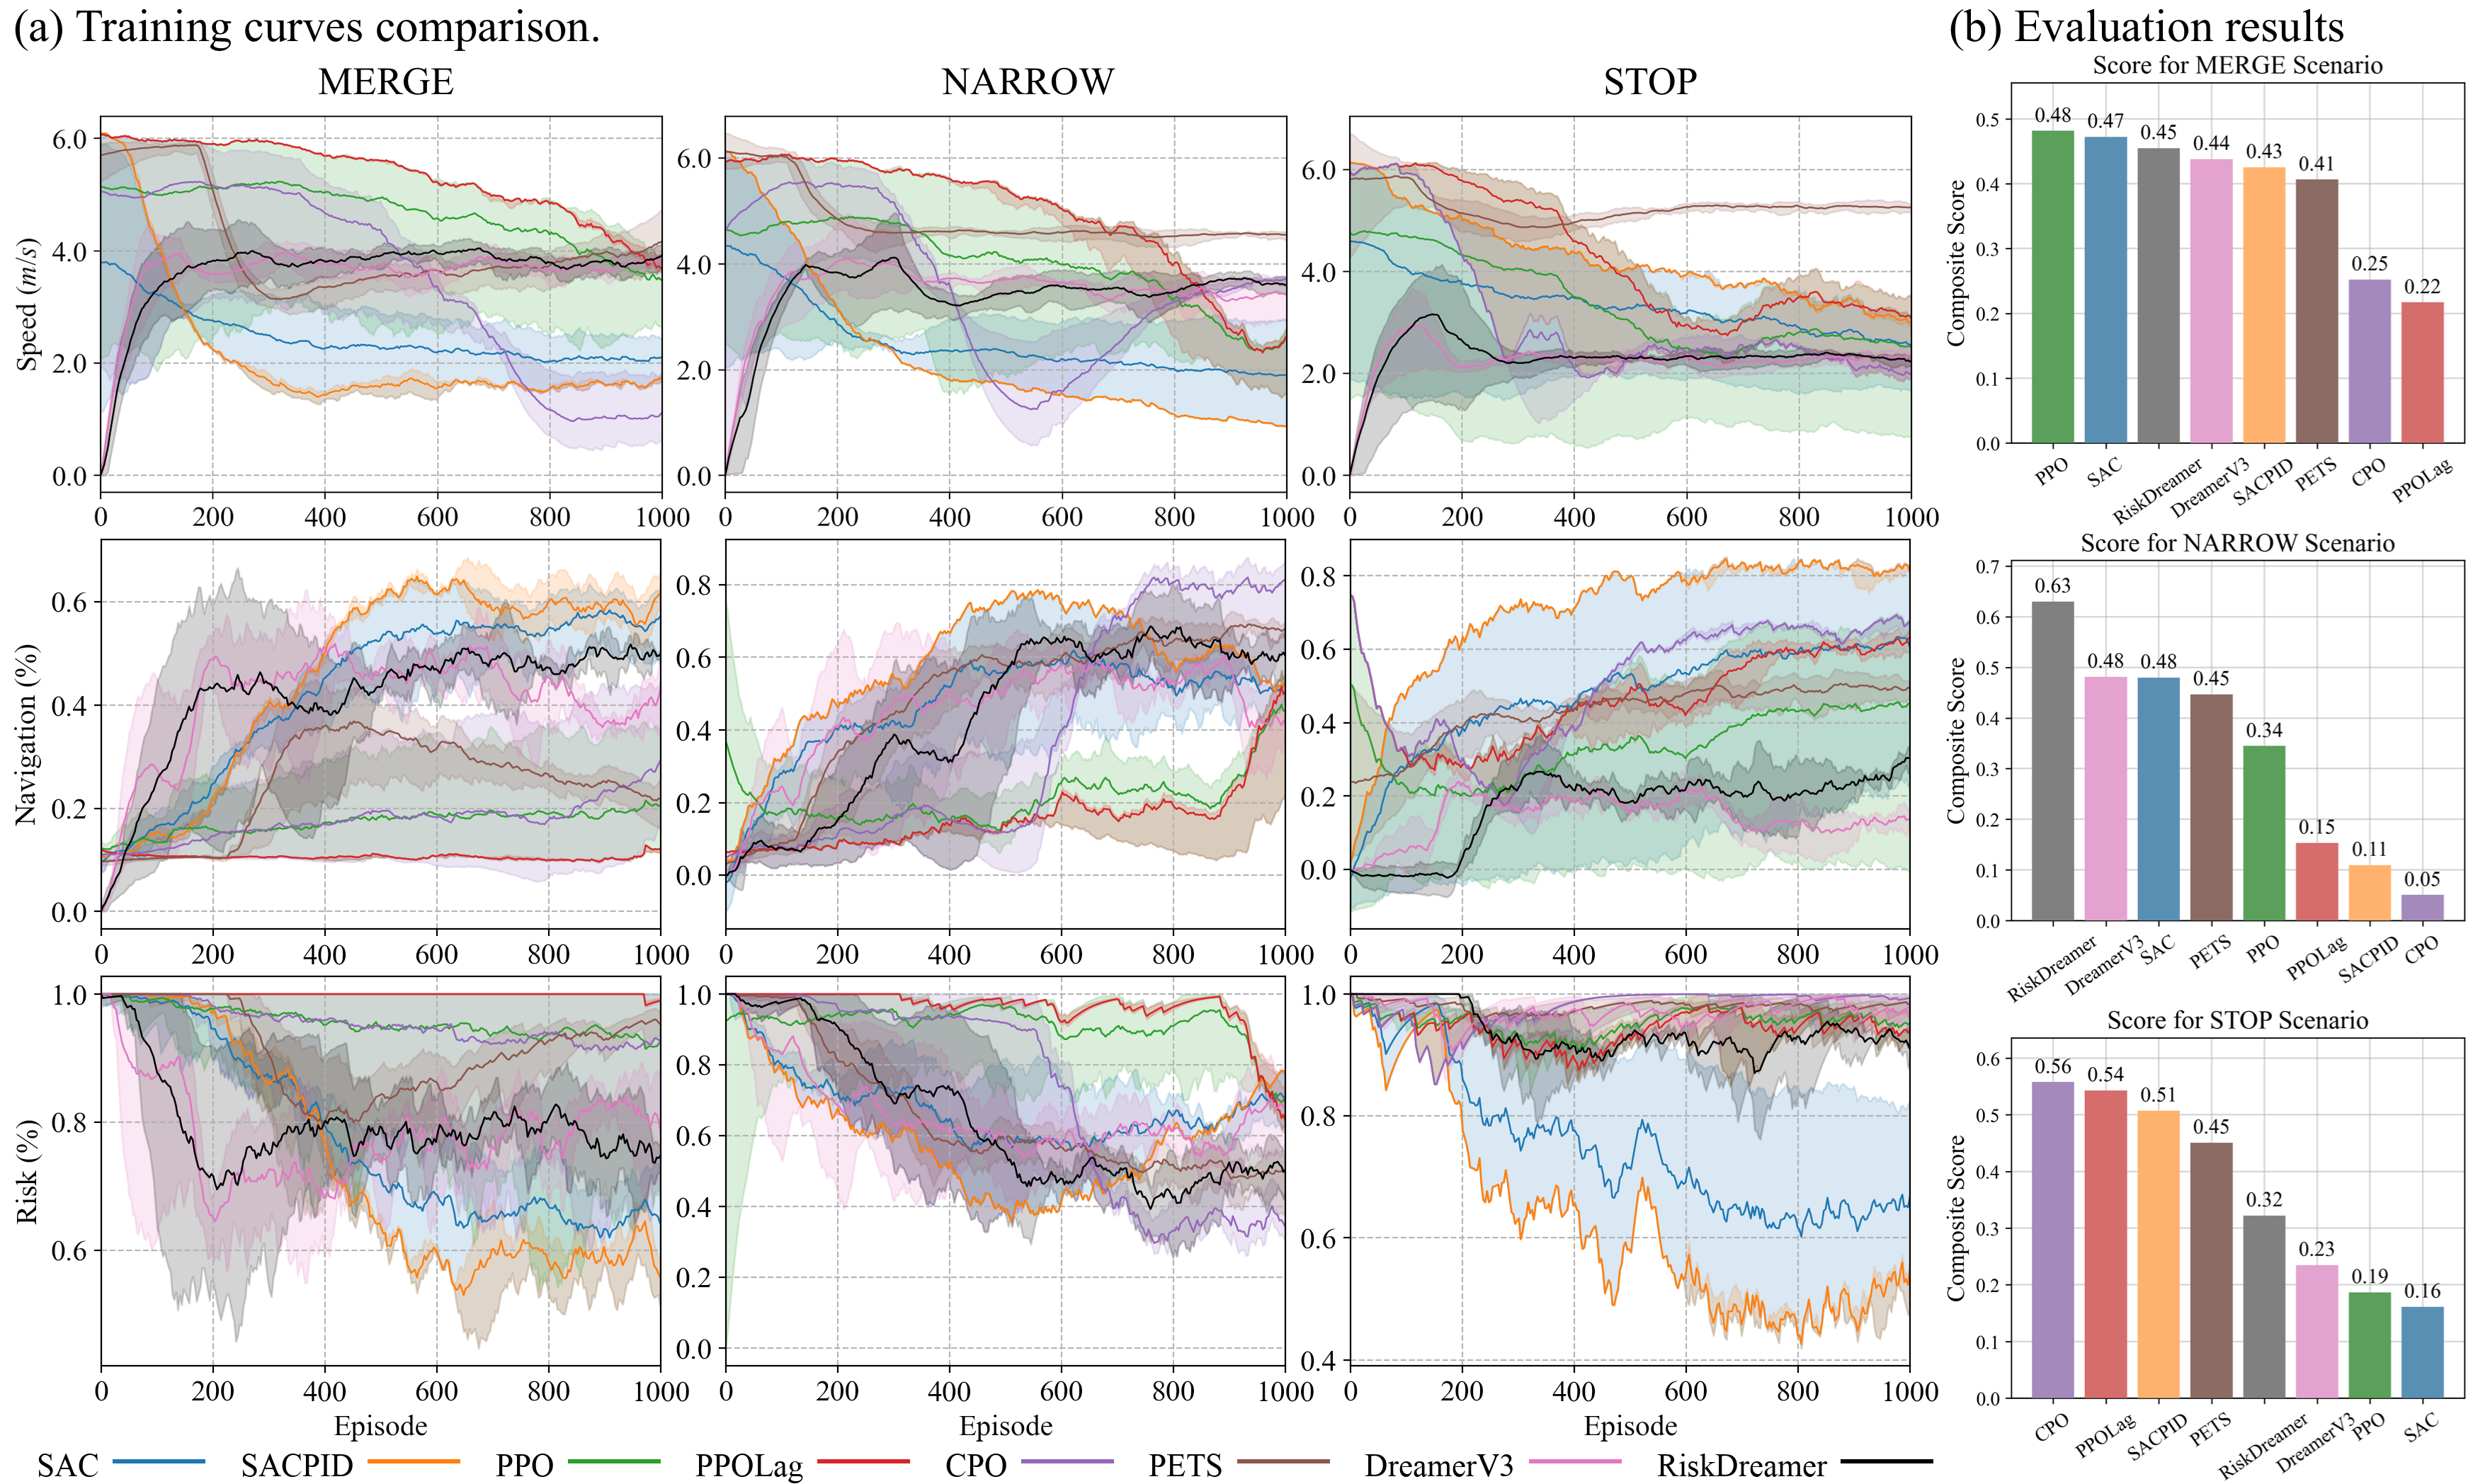
\includegraphics[width=\textwidth]{fig/train_curve.png}
    \caption{Results of different algorithm in the three scenarios. (a) Training curves comparison. (b) Evaluation results}
    \label{fig:train_curve}
\end{figure*}


\begin{figure*}[!htbp]
    \centering
    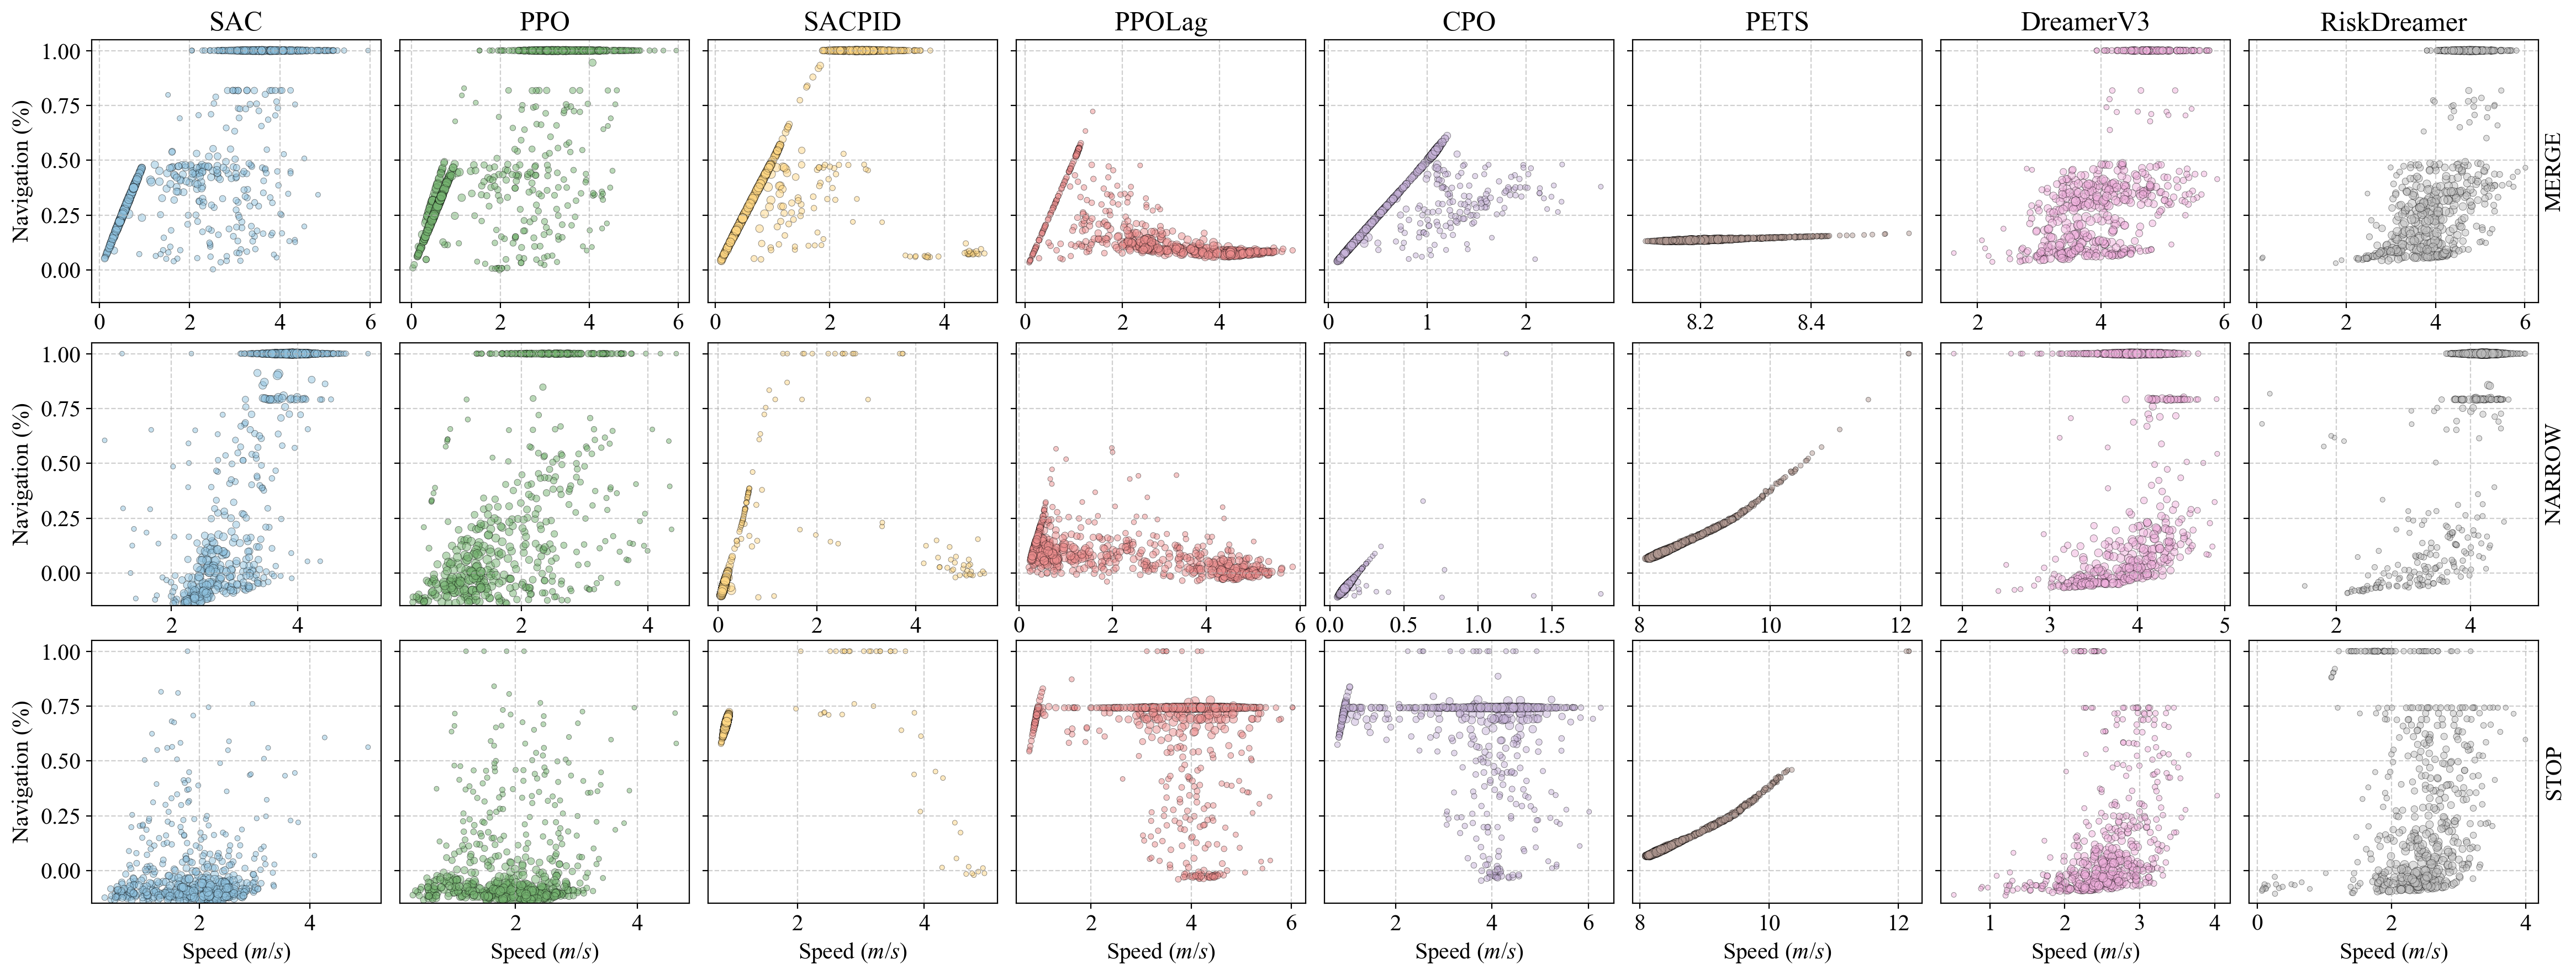
\includegraphics[width=\textwidth]{fig/algo_scatter_compare.png}
    \caption{Evaluation pattern of agent performance: Speed vs. Navigation. Bigger points indicate denser data point distributions.}
    \label{fig:eval}
\end{figure*}


\begin{table*}[tbp]
    \centering
    \caption{Performance comparison of different methods in multiple scenarios.}
    \label{table:comparison}
    \centering
    \setlength{\tabcolsep}{5pt}
    \begin{tabular}{p{1.4cm}m{1.6cm}p{0.78cm}p{0.78cm}p{0.78cm}p{0.78cm}p{0.78cm}p{0.78cm}p{0.78cm}p{0.78cm}p{0.78cm}p{0.78cm}p{0.78cm}p{0.78cm}}
        \toprule
        \textbf{Method} & \textbf{Metric} & \multicolumn{4}{c}{\textbf{MERGE Scenario}} & \multicolumn{4}{c}{\textbf{NARROW Scenario}} & \multicolumn{4}{c}{\textbf{STOP Scenario}} \\
        \cmidrule(lr){3-6} \cmidrule(lr){7-10} \cmidrule(lr){11-14}
         & & Mean & .Std & $\Delta$Value & $\Delta \%$ & Mean & .Std & $\Delta$Value & $\Delta \%$ & Mean & .Std & $\Delta$Value & $\Delta \%$ \\
        \midrule
        \multirow{4}{4pt}{SAC} & Navigation & \fbox{0.542} & 0.337 & +0.157 & $\uparrow$40.9\%  & \fbox{0.511} & 0.423 & +0.196 & $\uparrow$62.3\%  & 0.130 & 0.133 & -0.227 & $\downarrow$63.6\%  \\
         & Mean Speed & 2.467 & 1.419 & -0.836 & $\downarrow$25.3\%  & 3.252 & 0.726 & +0.145 & $\uparrow$4.7\%  & 1.872 & 0.735 & -1.350 & $\downarrow$41.9\%  \\
         & Risk & 0.448 & 0.498 & -0.147 & $\downarrow$24.7\%  & 0.644 & 0.479 & +0.084 & $\uparrow$14.9\%  & 0.998 & 0.045 & +0.168 & $\uparrow$20.2\%  \\
         & Score & \fbox{0.472} & 0.487 & +0.079 & $\uparrow$20.0\%  & 0.480 & 0.368 & +0.143 & $\uparrow$42.4\%  & 0.161 & 0.239 & -0.209 & $\downarrow$56.5\%  \\
        \midrule
        \multirow{4}{4pt}{PPO} & Navigation & \textbf{0.560} & 0.352 & +0.175 & $\uparrow$45.4\%  & 0.386 & 0.384 & +0.071 & $\uparrow$22.5\%  & 0.165 & 0.177 & -0.192 & $\downarrow$53.8\%  \\
         & Mean Speed & 2.389 & 1.418 & -0.915 & $\downarrow$27.7\%  & 1.988 & 0.905 & -1.119 & $\downarrow$36.0\%  & 1.898 & 0.746 & -1.324 & $\downarrow$41.1\%  \\
         & Risk & 0.400 & 0.490 & -0.195 & $\downarrow$32.7\%  & 0.734 & 0.442 & +0.174 & $\uparrow$31.0\%  & 0.992 & 0.089 & +0.162 & $\uparrow$19.5\%  \\
         & Score & \textbf{0.482} & 0.492 & +0.088 & $\uparrow$22.4\%  & 0.345 & 0.382 & +0.008 & $\uparrow$2.3\%  & 0.187 & 0.256 & -0.184 & $\downarrow$49.6\%  \\
        \midrule
        \multirow{4}{4pt}{SACPID} & Navigation & 0.521 & 0.360 & +0.136 & $\uparrow$35.4\%  & 0.125 & 0.197 & -0.190 & $\downarrow$60.2\%  & \textbf{0.665} & 0.118 & +0.309 & $\uparrow$86.6\%  \\
         & Mean Speed & 1.604 & 1.149 & -1.699 & $\downarrow$51.4\%  & 0.584 & 1.235 & -2.523 & $\downarrow$81.2\%  & 1.109 & 0.787 & -2.112 & $\downarrow$65.6\%  \\
         & Risk & \textbf{0.210} & 0.408 & -0.385 & $\downarrow$64.7\%  & \fbox{0.114} & 0.318 & -0.446 & $\downarrow$79.7\%  & \textbf{0.052} & 0.222 & -0.778 & $\downarrow$93.7\%  \\
         & Score & 0.425 & 0.427 & +0.032 & $\uparrow$8.1\%  & 0.110 & 0.395 & -0.227 & $\downarrow$67.5\%  & 0.507 & 0.250 & +0.137 & $\uparrow$37.0\%  \\
        \midrule
        \multirow{4}{4pt}{PPOLag} & Navigation & 0.171 & 0.139 & -0.214 & $\downarrow$55.7\%  & 0.095 & 0.093 & -0.220 & $\downarrow$70.0\%  & 0.583 & 0.253 & +0.226 & $\uparrow$63.5\%  \\
         & Mean Speed & 2.602 & 1.446 & -0.701 & $\downarrow$21.2\%  & 2.333 & 1.716 & -0.774 & $\downarrow$24.9\%  & \fbox{3.597} & 1.238 & +0.376 & $\uparrow$11.7\%  \\
         & Risk & 0.804 & 0.397 & +0.209 & $\uparrow$35.2\%  & 0.878 & 0.328 & +0.318 & $\uparrow$56.7\%  & 0.888 & 0.316 & +0.058 & $\uparrow$7.0\%  \\
         & Score & 0.217 & 0.445 & -0.176 & $\downarrow$44.8\%  & 0.154 & 0.519 & -0.183 & $\downarrow$54.4\%  & \fbox{0.543} & 0.412 & +0.172 & $\uparrow$46.6\%  \\
        \midrule
        \multirow{4}{4pt}{CPO} & Navigation & 0.313 & 0.163 & -0.072 & $\downarrow$18.6\%  & 0.065 & 0.049 & -0.250 & $\downarrow$79.2\%  & \fbox{0.607} & 0.240 & +0.251 & $\uparrow$70.3\%  \\
         & Mean Speed & 0.876 & 0.512 & -2.428 & $\downarrow$73.5\%  & 0.129 & 0.123 & -2.978 & $\downarrow$95.9\%  & 3.538 & 1.364 & +0.316 & $\uparrow$9.8\%  \\
         & Risk & \fbox{0.316} & 0.465 & -0.279 & $\downarrow$46.9\%  & \textbf{0.032} & 0.176 & -0.528 & $\downarrow$94.3\%  & \fbox{0.858} & 0.349 & +0.028 & $\uparrow$3.3\%  \\
         & Score & 0.252 & 0.191 & -0.141 & $\downarrow$35.9\%  & 0.051 & 0.051 & -0.286 & $\downarrow$85.0\%  & \textbf{0.558} & 0.442 & +0.187 & $\uparrow$50.6\%  \\
        \midrule
        \multirow{4}{4pt}{PETS} & Navigation & 0.139 & 0.006 & -0.246 & $\downarrow$63.8\%  & 0.166 & 0.116 & -0.149 & $\downarrow$47.2\%  & 0.171 & 0.118 & -0.185 & $\downarrow$52.0\%  \\
         & Mean Speed & \textbf{8.236} & 0.082 & +4.932 & $\uparrow$149.3\%  & \textbf{8.810} & 0.642 & +5.703 & $\uparrow$183.5\%  & \textbf{8.818} & 0.663 & +5.597 & $\uparrow$173.7\%  \\
         & Risk & 1.000 & 0.000 & +0.405 & $\uparrow$68.1\%  & 0.996 & 0.063 & +0.436 & $\uparrow$77.8\%  & 0.994 & 0.077 & +0.164 & $\uparrow$19.7\%  \\
         & Score & 0.406 & 0.025 & +0.013 & $\uparrow$3.3\%  & 0.447 & 0.209 & +0.110 & $\uparrow$32.6\%  & 0.451 & 0.216 & +0.080 & $\uparrow$21.7\%  \\
        \midrule
        \multirow{4}{4pt}{DreamerV3} & Navigation & 0.404 & 0.323 & +0.019 & $\uparrow$4.9\%  & 0.479 & 0.439 & +0.164 & $\uparrow$52.0\%  & 0.199 & 0.260 & -0.158 & $\downarrow$44.2\%  \\
         & Mean Speed & \fbox{4.136} & 0.766 & +0.832 & $\uparrow$25.2\%  & \fbox{3.893} & 0.457 & +0.786 & $\uparrow$25.3\%  & 2.554 & 0.501 & -0.668 & $\downarrow$20.7\%  \\
         & Risk & 0.810 & 0.393 & +0.215 & $\uparrow$36.2\%  & 0.640 & 0.480 & +0.080 & $\uparrow$14.2\%  & 0.962 & 0.191 & +0.132 & $\uparrow$15.9\%  \\
         & Score & 0.438 & 0.323 & +0.044 & $\uparrow$11.3\%  & \fbox{0.481} & 0.336 & +0.144 & $\uparrow$42.7\%  & 0.235 & 0.236 & -0.135 & $\downarrow$36.6\%  \\
        \midrule
        \multirow{4}{4pt}{RiskDreamer \\ \textbf{(Ours)}} & Navigation & 0.429 & 0.349 & +0.044 & $\uparrow$11.5\%  & \textbf{0.692} & 0.405 & +0.377 & $\uparrow$119.8\%  & 0.332 & 0.330 & -0.024 & $\downarrow$6.8\%  \\
         & Mean Speed & 4.120 & 0.832 & +0.816 & $\uparrow$24.7\%  & 3.867 & 0.601 & +0.760 & $\uparrow$24.5\%  & 2.386 & 0.638 & -0.836 & $\downarrow$25.9\%  \\
         & Risk & 0.770 & 0.421 & +0.175 & $\uparrow$29.5\%  & 0.444 & 0.497 & -0.116 & $\downarrow$20.7\%  & 0.898 & 0.303 & +0.068 & $\uparrow$8.2\%  \\
         &\cellcolor{lightgray}  Score &\cellcolor{lightgray}  0.455 &\cellcolor{lightgray}  0.349 &\cellcolor{lightgray}  +0.061 &\cellcolor{lightgray}  $\uparrow$15.6\%  &\cellcolor{lightgray}  \textbf{0.630} &\cellcolor{lightgray}  0.336 &\cellcolor{lightgray}  +0.293 &\cellcolor{lightgray}  $\uparrow$86.8\%  &\cellcolor{lightgray}  0.322 &\cellcolor{lightgray}  0.300 &\cellcolor{lightgray}  -0.048 &\cellcolor{lightgray}  $\downarrow$13.1\%  \\
        \midrule
    \end{tabular}
\end{table*}




\subsection{Benchmark and Metrics}



To evaluate RiskDreamer, we benchmark its performance against advanced RL methods, categorized into following groups:

\subsubsection{Established RL Methods} 

\textbf{Proximal Policy Optimization (PPO)}\cite{PPO}: A widely used RL algorithm employing policy clipping for stable training. PPO is efficient, requires minimal hyperparameters, and generalizes well across continuous and discrete action spaces.

\textbf{Soft Actor-Critic (SAC)}\cite{SAC}: An off-policy algorithm using maximum entropy policy gradients for enhanced exploration and sample efficiency. SAC exhibits stable convergence and robust performance, especially in continuous action spaces.


\subsubsection{Vanilla Safe RL Methods}

    \textbf{Conservative Policy Optimization (CPO)}\cite{CPO}: A foundational trust region safe RL method. CPO enforces safety by limiting policy updates within a trust region, providing a conservative approach for risky environments.

    \textbf{PPO-Lagrangian (PPO-Lag)}\cite{PPO}: Extends PPO with a Lagrangian term to balance reward maximization and constraint satisfaction. Effective for constrained optimization.

    \textbf{Soft Actor-Critic with PID Controller (SACPID)}\cite{SACPID}:  Enhances SAC with a PID controller to mitigate oscillations in Lagrangian methods, leading to more stable constrained optimization.

\subsubsection{Model-Based Safe RL Method}
    \textbf{Constrained Cross-Entropy Method for Policy Evolution on Trajectory Search (PETS)}\cite{CCEPETS}: A gradient-free, population-based method using cross-entropy optimization. PETS refines policies based on performance and constraint satisfaction via trajectory sampling.

\subsubsection{SOTA World Model Method}
    \textbf{DreamerV3}\cite{dreamerv3}:  State-of-the-art multi-task world model. DreamerV3 learns environment dynamics and improves policies through imagination, enabling robust learning across diverse environments.


The performance of each algorithm was evaluated across MERGE, NARROW, and STOP scenarios. The evaluation metrics are defined as follows:

    \begin{enumerate}
        \item \textbf{Navigation:} Percentage of navigation distance covered. Higher value indicates better route following.
        \item \textbf{Mean Speed:} Average speed of the ego vehicle during the episode. Reflects driving efficiency.
        \item \textbf{Risk:} Average risk across episodes (0: no collision, 1: collision). 
        \item \textbf{Composite Score:}  $0.7 \times \text{Navigation} + 0.3 \times \frac{\text{Mean Speed}}{\text{Max Speed}}$.  
    \end{enumerate}    

\subsection{Results Analysis}

This section presents the results of the training and evaluation of the RiskDreamer and the benchmarked methods.
Fig. \ref{fig:train_curve} (a) presents the training curves for key performance indicators. Fig. \ref{fig:train_curve} (b) summarizes the composite scores achieved by each algorithm in each scenario. Table \ref{table:comparison} provides detailed quantitative results for each metric across all scenarios and algorithms. Fig. \ref{fig:eval} shows the distribution of evaluation scores in Speed vs. Navigation coordinates.



\textbf{Analysis of Training Curves}: As shown in Fig. \ref{fig:train_curve} (a), in the MERGE scenario, RiskDreamer demonstrates stable improvements in navigation success rate, with its risk level gradually decreasing and stabilizing. The baseline DreamerV3 initially performs similarly to RiskDreamer, but its performance declines as training continues. On the other hand, SAC and SACPID excel at reducing risk but demonstrate conservative training results in their actions, leading to slow speeds.

In the NARROW scenario, the navigation difficulty is reduced. While maintaining its speed, RiskDreamer shows continuous improvement in navigation success rate. The baseline DreamerV3 still experiences performance degradation in the later stages of training. PPO and SAC show improvement in navigation but maintain low speeds. However, they often exhibit high risk levels. PETS maintains high speed but encounters difficulties in navigation and maintains high risk. CPO sometimes achieves low risk and high speed, but training results fluctuate significantly.

In the STOP scenario, navigation difficulty is highest. RiskDreamer demonstrates speed reduction and moderate improvement in navigation success rate. Although there is improvement compared to the baseline DreamerV3, it performs mediocrely in this scenario. SAC and SACPID show rapid initial risk reduction, followed by stabilization at a higher level. PETS initially achieves high speed but cannot park reliably, resulting in sustained high risk.


\textbf{Analysis of Evaluation Results:}
As shown in Fig. \ref{fig:train_curve} (b), the composite score provides an overall performance measure that balances speed, navigation, and risk. In the MERGE scenario, PPO, SAC, and RiskDreamer achieve comparable composite scores, indicating a balance between different objectives. PETS and PPOLag show lower scores due to the trade-offs between speed and safety.

In the NARROW scenario, RiskDreamer achieves the highest composite score, significantly outperforming other algorithms. Compared to DreamerV3, it shows a \SI{31.25}{\%} improvement, though DreamerV3 also achieves a competitive score. CPO again shows lower scores, highlighting its difficulty in navigating confined spaces while maintaining safety. CPO and PPOLag show negative composite scores, indicating poor overall performance.

In the STOP scenario, CPO achieves the highest composite score, reflecting its ability to prioritize safety. PPOLag and SACPID also achieve relatively high scores. RiskDreamer demonstrates a moderate composite score, showing a \SI{29.13}{\%} improvement compared to the baseline DreamerV3, though neither performs at the top of the rankings.

\textbf{Quantitative Analysis:}
The quantitative results in table \ref{table:comparison} confirm the observations from the charts. RiskDreamer performs well in the MERGE scenario, achieving an average speed (4.12 \si{m/s}) and a respectable navigation score (0.43). While its risk is moderate (0.77), its final composite score (0.426) is competitive. In the NARROW scenario, RiskDreamer performs the best, achieving a high average speed (3.87 \si{m/s}) and the highest navigation score (0.69), leading to the highest composite score (0.63).

In the STOP scenario, RiskDreamer exhibits a lower average speed (2.39 \si{m/s}) but maintains a reasonable navigation score (0.33) and a relatively high risk (0.90), resulting in a lower composite score (0.30) compared to safety-focused algorithms like CPO and PPOLag. PETS consistently achieves the highest average speeds across all scenarios but exhibits extremely low navigation scores and near-perfect risk, leading to low composite scores, indicating its failure to effectively navigate and prioritize safety. Conversely, CPO and PPOLag tend towards lower speeds but prioritize safety, achieving high risk scores in the STOP scenario but lower composite scores in the MERGE and NARROW scenarios due to their conservative behavior.

\textbf{Evaluation Pattern Analysis:}
Fig. \ref{fig:eval} provides a visual representation of the evaluation results in Speed vs. Navigation coordinates. Smaller scatter points represent denser sampling regions, reflecting the distribution of algorithm performance at varying speeds and navigation success rates. There are noticeable differences in the point cloud distributions of each algorithm across different scenarios. The distributions of SAC and PPO are similar: there's a higher concentration of points in the regions with lower navigation success rates (representing early collisions or failures), while there's also a linear distribution of points clustered when the navigation success rate approaches 1. This suggests that they either tend to fail early on or can successfully achieve the final goal. DreamerV3 and RiskDreamer also exhibit similar trends, but their point distribution in the medium navigation range is slightly elevated, and as speed increases, navigation completion also increases accordingly. Compared to the baseline algorithm DreamerV3, RiskDreamer achieves a linear distribution at high success rates at a faster speed, indicating it possesses a certain advantage in balancing risk and efficiency.

In the context of safe reinforcement learning, methods such as SACPID, PPOLag and CPO, their distribution areas in the figure are observed to be generally lifted towards the middle. This implies that a relative balance has been achieved between speed and success rate, but the number of full navigations (success rate of 1) has decreased, indicating that these algorithms sacrifice some extreme optimal performance while improving safety. It's worth noting that, although PETS has a noticeable distribution in the high-speed region, it can hardly complete navigation, and its performance is severely limited.

\textbf{Discussion:}
RiskDreamer demonstrates the ability to adapt its behavior across different scenarios. In the MERGE and NARROW scenarios, it strikes a good balance between speed and navigation while maintaining reasonable risk levels. While its composite score in the STOP scenario is inferior compared to safety-focused RL algorithms, it still outperforms the baseline DreamerV3. The results suggest that RiskDreamer avoids the overly conservative behavior of some safety RL algorithms and the reckless behavior of purely performance-driven approaches. The ablation study in the next section will further explore the effectiveness of RiskDreamer's dynamic risk-entropy balancing mechanism.


\subsection{Ablation Study}


To evaluate the contribution of individual components within the RiskDreamer framework, we conducted a series of ablation studies. These studies specifically assessed the impact of the entropy and risk-balancing mechanisms, as well as the effect of the online planning horizon on the batch planning process.



\begin{figure*}[!htbp]
    \centering
    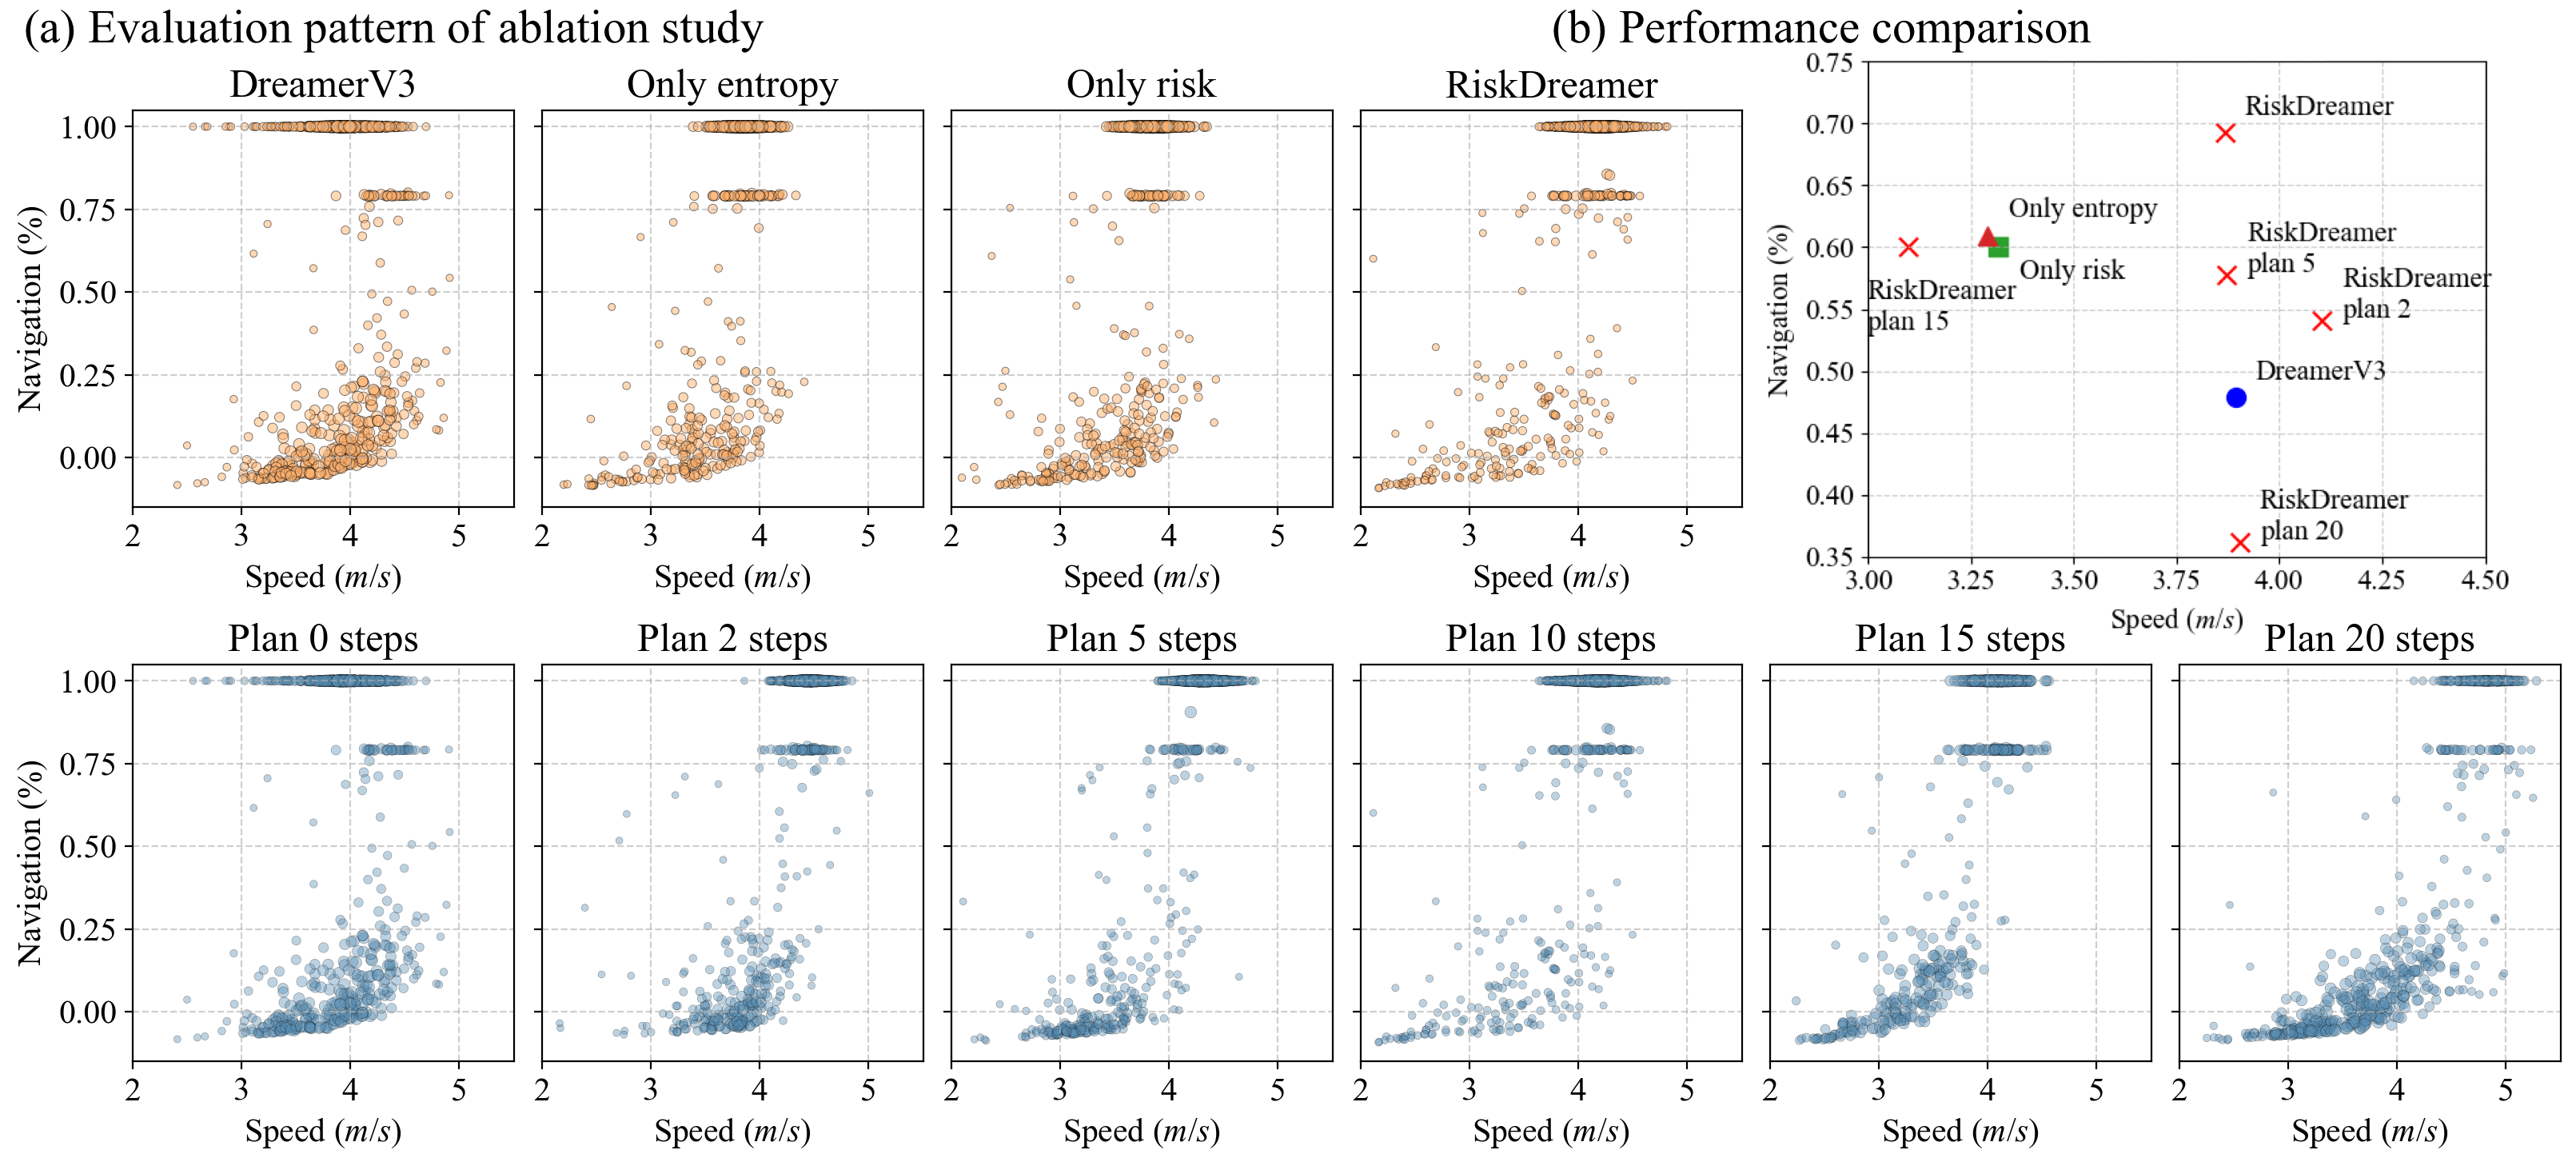
\includegraphics[width=\textwidth]{fig/abafig.png}
    \caption{Results of ablation study (a) Evaluation pattern (b) Performance comparison}
    \label{fig:aba_fig}
\end{figure*}

\begin{table}[!ht]
    \caption{Impact of Entropy and Risk Balancing}
    \label{table:ablation_entropy_risk}
    \centering
    \begin{tabular}{lcccc}
    \toprule
    Algorithm & Speed (Std.) & Navigation (Std.) & Risk (Std.) & Score \\
    \midrule
    \rowcolor{lightgray} RiskDreamer & 3.87 (0.60) & \textbf{0.69} (0.40) & \textbf{0.44} (0.50) & \textbf{0.63} \\
    Only entropy term & 3.29 (0.95) & 0.61 (0.42) & 0.63 (0.48) & 0.55 \\
    Only risk term & 3.32 (0.90) & 0.60 (0.43) & 0.61 (0.49) & 0.54 \\
    DreamerV3 & \textbf{3.89} (0.46) & 0.48 (0.44) & 0.64 (0.48) & 0.48 \\
    \bottomrule
    \end{tabular}
\end{table}



\textbf{Impact of Entropy and Risk Balancing:}
Table \ref{table:ablation_entropy_risk} presents two ablated versions: one using only the entropy balancing term in the action expansion and the other using only the risk balancing term. The full RiskDreamer model achieves the highest overall score (0.63), outperforming both ablated versions and the baseline DreamerV3. RiskDreamer demonstrates superior performance in Navigation (0.69) and Risk (0.44), indicating a more effective balance between task completion and risk mitigation. Although the ablated versions with only entropy or only risk balancing show slightly improved navigation score compared to DreamerV3, they still underperform relative to RiskDreamer and exhibit higher risk values (0.63 and 0.61, respectively). DreamerV3, which does not include explicit entropy or risk balancing, achieves the highest Mean Speed (3.89) but performs poorly in Navigation (0.48) and incurs the highest Risk (0.64), resulting in the lowest overall Score (0.48). Fig. \ref{fig:aba_fig} (a) shows that using only the entropy or risk term reduces the low-speed portion of completed navigation clusters, whereas the full RiskDreamer implementation increases the high-speed portion of these clusters. Fig. \ref{fig:aba_fig} (b) illustrates that both single-term versions produce comparable outcomes by decreasing speed while improving navigation success.

\begin{table}[!ht]
    \caption{Impact of the Number of Planning Branches}
    \label{table:ablation_plan_len}
    \centering
    \begin{tabular}{lcccc}
    \toprule
    Horizon ($H$) & Speed (Std.) & Navigation (Std.) & Risk (Std.) & Score \\
    \midrule
    \rowcolor{lightgray} \textbf{$H$ = 10 (Chosen)} & 3.87 (0.60) & \textbf{0.69} (0.40) & \textbf{0.44} (0.50) & \textbf{0.63} \\
    $H$ = 5 & 3.87 (0.59) & 0.58 (0.44) & 0.54 (0.50) & 0.55 \\
    $H$ = 15 & 3.10 (1.15) & 0.60 (0.41) & 0.75 (0.43) & 0.54 \\
    $H$ = 2 & \textbf{4.10} (0.50) & 0.54 (0.44) & 0.60 (0.49) & 0.53 \\
    $H$ = 0 & 3.89 (0.46) & 0.48 (0.44) & 0.64 (0.48) & 0.48 \\
    $H$ = 20 & 3.90 (0.87) & 0.36 (0.40) & 0.80 (0.40) & 0.40 \\
    \bottomrule
    \end{tabular}
\end{table}

\textbf{Influence of Planning horizon length:}
We further investigated the impact of the length of planning horizons employed in our batch planning approach. Table \ref{table:ablation_plan_len} shows RiskDreamer's performance under different planning horizon lengths, ranging from 0 (equivalent to DreamerV3's single-step action selection) to 20. The results indicate that the length of planning horizon significantly affects performance. RiskDreamer with a planning length of 10, our chosen configuration, achieved the best overall Score (0.63), Navigation (0.69), and Risk (0.44). Reducing the planning length to 5 still maintains a competitive Mean Speed (3.87) but leads to a noticeable decrease in Navigation (0.58) and an increase in Risk (0.54), resulting in a lower Score (0.55). Conversely, increasing the planning length beyond 10, such as to 15 and 20, results in degradation of all metrics except for Mean Speed in the case of plan = 20. Specifically, with planning lengths of 15 and 20, we observe a significant increase in Risk (0.75 and 0.80 respectively) and a substantial drop in Navigation (0.60 and 0.36 respectively), leading to lower Scores (0.54 and 0.40). Interestingly, while a very short planning length of 2 leads to the highest Mean Speed (4.10), it also results in compromised Navigation (0.54) and Risk (0.60), and a lower Score (0.53) compared to plan = 10. The case with plan length 0, which is equivalent to acting without planning (similar to DreamerV3), yields the lowest Score (0.48). As shown in Fig. \ref{fig:aba_fig} (a) Evaluation pattern, even plan 2 steps can reduce linear clustering in the low-speed region, with bottom collision clustering being an exception. Furthermore, except for step 15, the model's performance speed tends to increase as steps increase. Fig. \ref{fig:aba_fig} (b) Performance comparison shows increased navigation for all except plan 20.




\section{Conclusion}
\label{sec:conclusion}
In this paper, we introduced RiskDreamer, a novel model-based reinforcement learning framework that leverages batch planning in a latent space to dynamically balance risk, entropy, and expected reward. By extending the action space to output these balancing factors directly, our approach addresses the limitations of fixed-parameter risk allocation and overcomes the shortcomings of overly simplified or homogeneous traffic simulations. The trustworthy traffic scenario generation framework further reinforces the realism of the simulation environment by calibrating diverse traffic agents' behaviors to match real-world statistics.
\subsection{Evaluation Results}
The experimental evaluations across three typical autonomous driving scenarios demonstrate the effectiveness of the proposed RiskDreamer framework. In the MERGE scenario, RiskDreamer achieves a competitive composite score by balancing speed, navigation success, and risk, showcasing its ability to navigate complex merging situations without being overly conservative or reckless. The NARROW scenario further highlights RiskDreamer's capability in challenging environments, where it achieves the highest navigation score and a strong overall composite score, indicating effective maneuvering in constrained spaces. While in the STOP scenario, safety-focused algorithms achieved higher composite scores due to their emphasis on minimizing risk, RiskDreamer still demonstrated its improvements against baseline DreamerV3. Compared to baseline methods, RiskDreamer exhibits a more adaptive behavior, avoiding the high-risk tendencies of purely performance-driven approaches like PETS and the overly cautious nature of some SafeRL methods such as CPO and PPOLag in dynamic scenarios. The quantitative analysis further supports these observations, confirming RiskDreamer's ability to dynamically adjust its behavior based on the specific scenario demands.

\subsection{Limitations and Future Work}
Despite RiskDreamer's promising performance, there are several limitations and future research directions need to be taken into consideration. Firstly, due to computational constraints, our current implementation chooses a state-based environment representation.  Future work could explore richer, more realistic perception by incorporating vision-based or multi-modal sensory inputs, enhancing the agent's understanding of complex traffic scenarios. Secondly, while our trustworthy traffic scenario generator improves realism, SUMO remains a simplified traffic simulation environment with a relatively limited dataset.  Future research could integrate larger-scale, real-world trajectory datasets and explore more advanced simulators such as CARLA to further enhance the fidelity of the training and evaluation environment.  Finally, to more comprehensively validate RiskDreamer's real-world applicability and human-vehicle interaction, future studies should incorporate human-in-the-loop evaluations using driving simulators, bridging the gap between simulation and real-world driving scenarios.


\ifCLASSOPTIONcaptionsoff
  \newpage
\fi

\bibliographystyle{IEEEtran}
\bibliography{bibtex/bib/IEEEabrv.bib,bibtex/bib/IEEEexample.bib}{}
% or if you just want to reserve a space for a photo:

\vspace{-5 mm} 
\begin{IEEEbiography}[{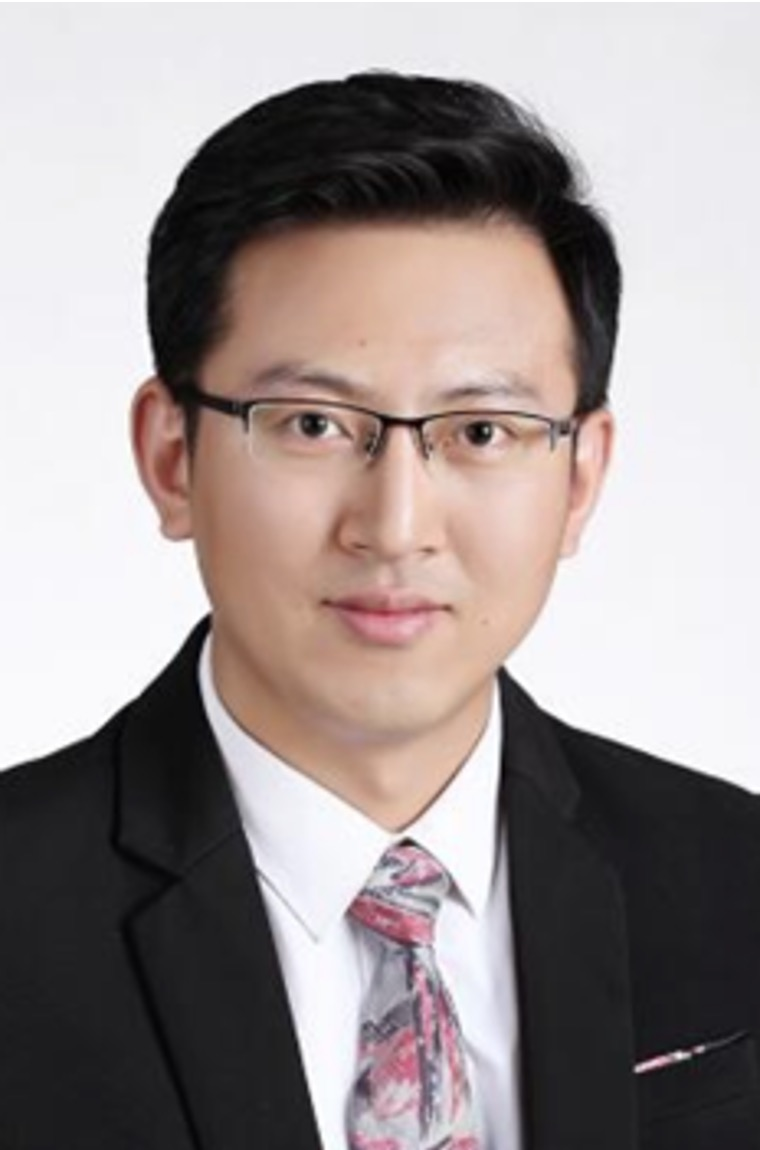
\includegraphics[width=1.02in,keepaspectratio,trim=0 2in 0 0,clip]{biography/liu.jpg}}]{Qingchao Liu }
    received the Ph.D. degree from Southeast University, Nanjing, China, in 2015. He joined the Automotive Engineering Research Institute, Jiangsu University, Zhenjiang, where he is currently working as an Associate Professor. His research interests include Driving behavior analysis, path planning, autonomous vehicle, cooperative adaptive cruise control, traffic flow theory, and intelligent transportation systems. He concurrently serves as a member of the American TRB Artificial Intelligence Subcommittee, a member of the China Society of Automotive Engineers, a member of the China Intelligent Transportation Association, and a senior visiting scholar at Nanyang Technological University in Singapore.
    \end{IEEEbiography}
    
    % if you will not have a photo at all:
    \begin{IEEEbiography}[{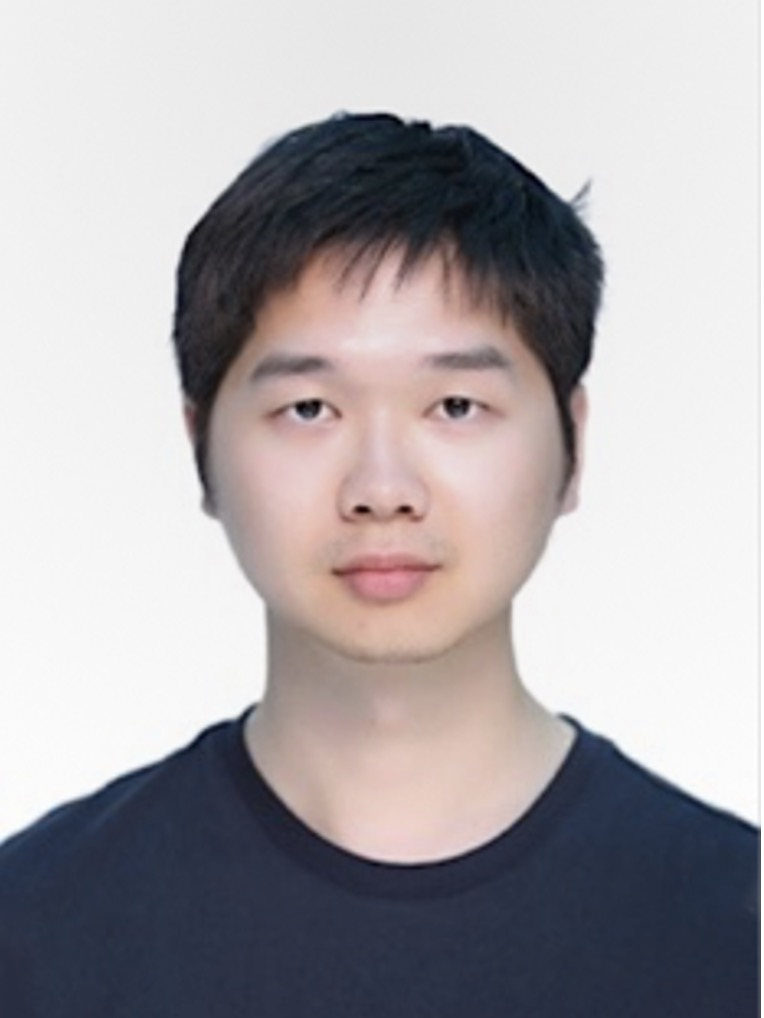
\includegraphics[width=1.02in,keepaspectratio,clip]{biography/gao.jpg}}]{Chengzhi Gao}
    received the bachelor degree in Information and Computing Science from the Anhui Agricultural University in 2022. He is currently pursuing a postgraduate degree in transportation engineering with Jiangsu University, China. His research interests include vehicular platoon control, traffic simulation and intelligent transportation systems. He is currently the deputy leader of the Waliang Lake Ecological Observation Team.
    \end{IEEEbiography}
       % \vspace{-5 mm} 
    \begin{IEEEbiography}[{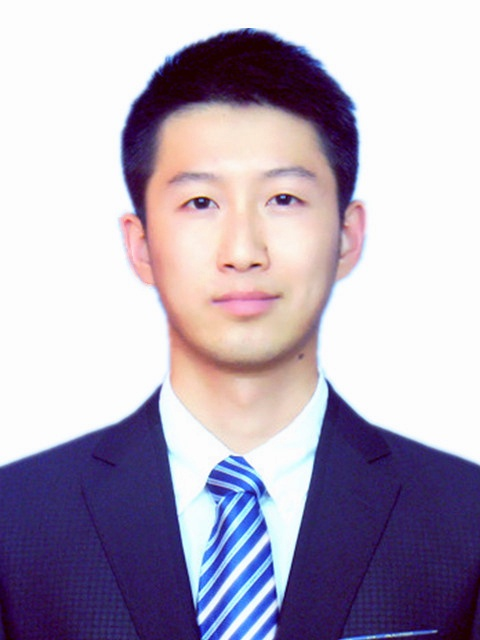
\includegraphics[width=1.02in,keepaspectratio,clip]{biography/hxk.jpg}}]{Xiangkun He}
        (Member, IEEE) is currently a UESTC 100 Young Professor at the University of Electronic Science and Technology of China. Previously, he was a Research Fellow at Nanyang Technological University, Singapore, and served as a Senior Research Scientist at Huawei Noah's Ark Lab from 2019 to 2021. He earned his Ph.D. in 2019 from the School of Vehicle and Mobility at Tsinghua University. He has authored over 50 papers in top-tier journals and conferences, such as TPAMI, TNNLS, TITS, TRC, and Engineering, and holds 8 granted patents. His research interests include reinforcement learning, trustworthy AI, autonomous vehicles, and robotics. He has received many awards and honors, selectively including the Tsinghua University Outstanding Doctoral Dissertation Award in 2019, Best Paper Finalist at IEEE ICMA 2020, Huawei Major Technological Breakthrough Award in 2021, Best Paper Runner-Up Award at CVCI 2022, and Runner-Up in the Intelligent Algorithm Final of the 2022 Alibaba Global Future Vehicle Challenge. He serves as a reviewer for over 50 renowned journals and conferences and was also a member of the award committee for the Autonomous Driving Control Benchmark Challenge at IEEE CDC 2023.
    \end{IEEEbiography} 
    % insert where needed to balance the two columns on the last page with
    % biographies
    %\newpage
    % \vspace{-5 mm} 
    \begin{IEEEbiography}[{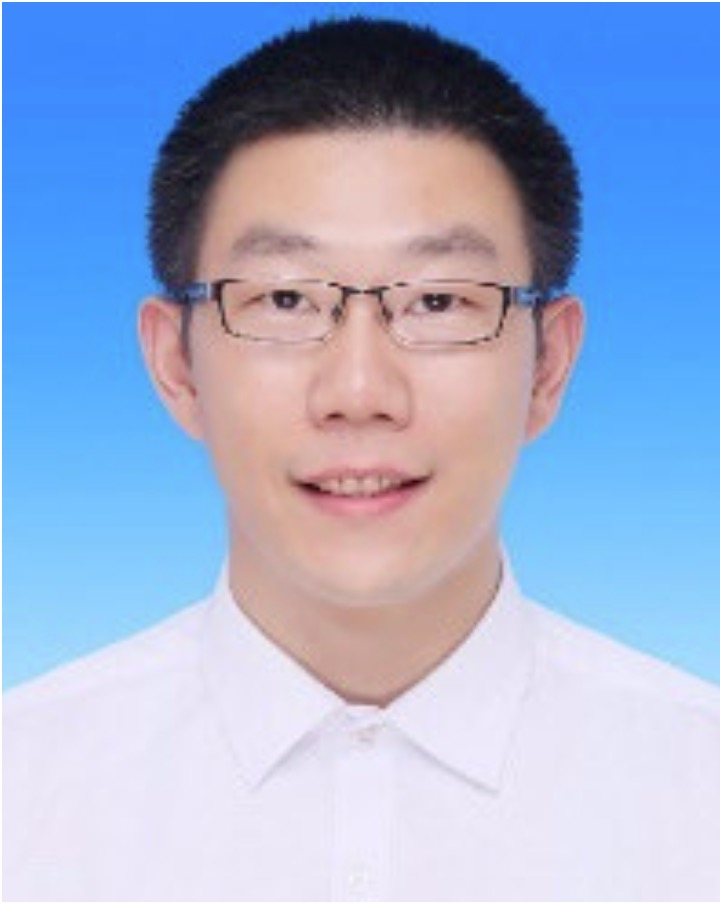
\includegraphics[width=1.02in,keepaspectratio,clip]{biography/wang.jpg}}]{Hai Wang}
        (Senior Member, IEEE) received the B.S., M.S., and Ph.D. degrees from the School of Instrument Science and Engineering, Southeast University, Nanjing, China, respectively. In 2012he joined the School of Automotive and Traffic Engineering at Jiangsu University, where, he is currently working as a Professor. He has authored or coauthored more than 50 papers in the field of machine vision-based environment sensing for intelligent vehicles. His research interests include computer vision, intelligent transportation systems and intelligent vehicles. 
    \end{IEEEbiography}
       
    % \vspace{-5 mm} 
    \begin{IEEEbiography}[{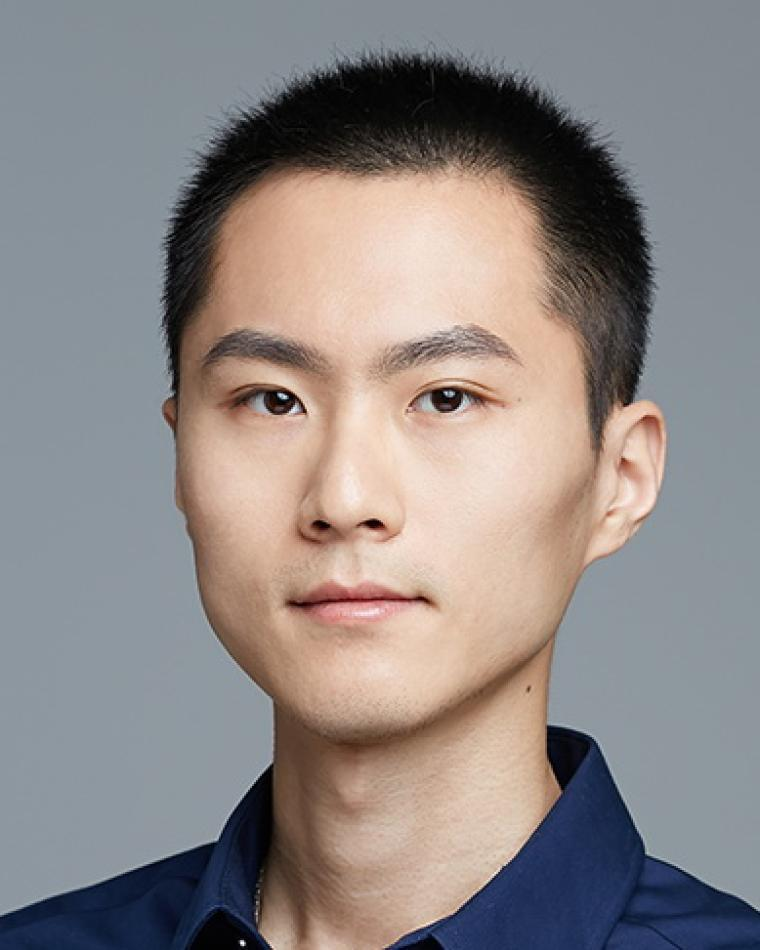
\includegraphics[width=1.02in,keepaspectratio,clip]{biography/lv.png}}]{Chen Lv}
        (Senior Member. IEEE) received the Ph.D. degree from the Department of Automotive Engineering, Tsinghua University China in 2016From 2014 to 2015, he was a joint Ph.D. Researcher with the EECS Department, University of California at Berkeley. He is currently an Assistant Professor with Nanyang Technology University, Singapore. His research interests include cyber-physical systems, hybrid systems, advanced vehicle control, and intelligence, where he has contributed over 90 articles and holds 12 granted Chinese patents. He received the Highly Commended Paper Award of IMechE, U.K., in 2012, the National Fellowship for Doctoral Student in 2013, the NSK Outstanding Mechanical Engineering ward in 2014, the China SAE Outstanding Paper Award. in 2015, the 1st Class Award of China Automotive Industry Scientific and Technological Invention in 2015, the Tsinghua University Outstanding Doctoral Thesis Award in 2016, and the IV2018 Best Workshop/Special Issue Paper Award. He serves as a Guest Editor for IEEE Intelligent Transportation Systems Magazine, IEEE/ASME TRANSACTIONS ON MECHATRONICS, and Applied Energy, and an Associate Editor/Editorial.
    \end{IEEEbiography} 
    % \vspace{-5 mm} 
    \begin{IEEEbiography}[{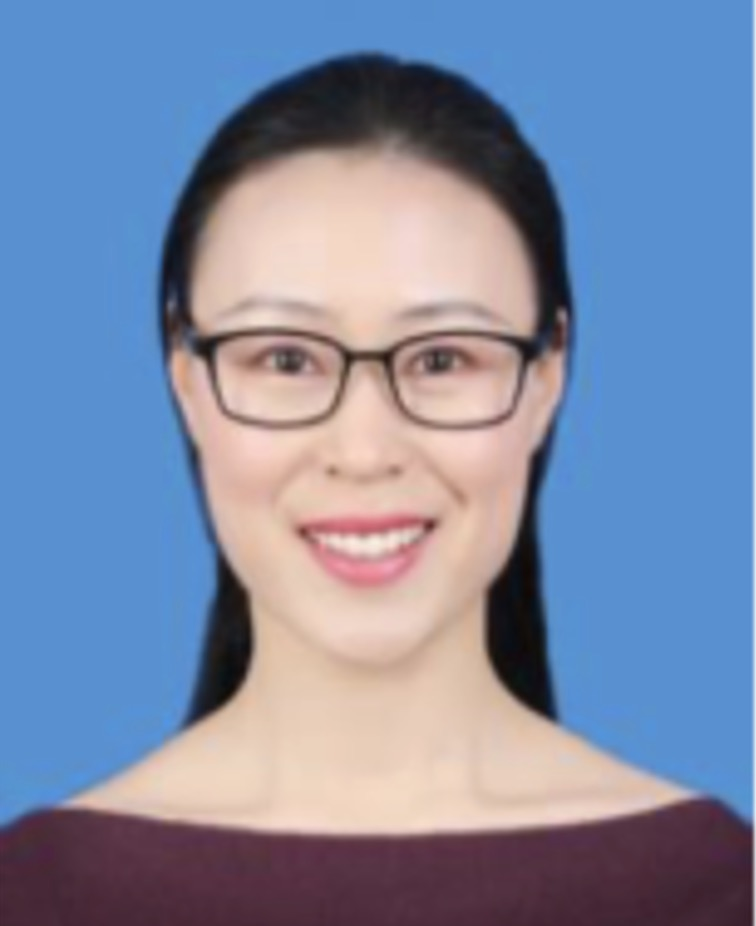
\includegraphics[width=1.02in,keepaspectratio,clip]{biography/cai.jpg}}]{Yingfeng Cai}
        (Senior Member, IEEE) received the B.S., M.S., and Ph.D. degrees from the School of Instrument Science and Engineering, Southeast University, Nanjing. China. In 2013, she joined the Automotive Engineering Research Institute, Jiangsu University, as a Professor. Her research interests include computer vision, intelligent transportation systems. And intelligent automobiles.
    \end{IEEEbiography}
    
    %     % \vspace{-5 mm} 
    \begin{IEEEbiography}[{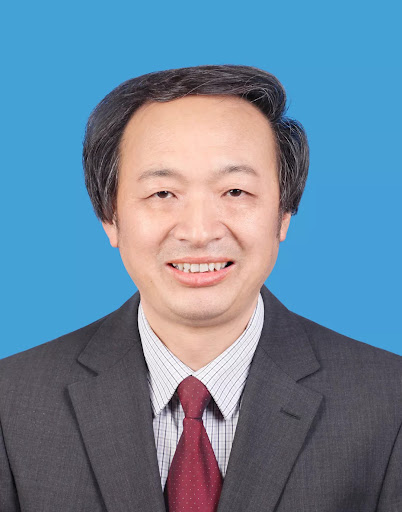
\includegraphics[width=1.02in,keepaspectratio,clip]{biography/chen.jpg}}]{Long Chen}
        received the B.Sc. and Ph.D. degrees in mechanical engineering from Jiangsu University, Zhenjiang, China, in 1982 and 2006, respectively. He is currently a Professor with the Automotive Engineering Research Institute, Jiangsu University Zhenjiang. His research interests include electric vehicles, electric drives, simulation and control of vehicle dynamic performance, vehicle operation, and transport planning.
    \end{IEEEbiography}


    % You can push biographies down or up by placing
    % a \vfill before or after them. The appropriate
    % use of \vfill depends on what kind of text is
    % on the last page and whether or not the columns
    % are being equalized.
    % \vfill

% 使用空白图像作为占位符
% \begin{IEEEbiography}[{\includegraphics[width=1.02in,keepaspectratio]{example-image}}]{Michael Smith}
%     received the Ph.D. degree from the University of California, Los Angeles (UCLA), USA, in 2016. He joined the Mechanical Engineering Department at XYZ University, USA, where he is currently working as an Associate Professor. His research interests include autonomous vehicle technology, human-machine interaction, path planning, traffic optimization, and intelligent transportation systems. He concurrently serves as a member of the SAE Technical Committee on Autonomous Systems, a member of the American Society of Mechanical Engineers, and a visiting scholar at ABC University, UK.
% \end{IEEEbiography}

% % 使用空白图像作为占位符
% \begin{IEEEbiography}[{\includegraphics[width=1.02in,keepaspectratio]{example-image}}]{Alex Johnson}
%     received the bachelor degree in Applied Mathematics from the University of Texas at Austin in 2021. He is currently pursuing a postgraduate degree in transportation systems engineering at XYZ University, USA. His research interests include vehicle platoon optimization, traffic flow simulation, and smart transportation networks. He currently leads the Sustainable Mobility Research Group.
% \end{IEEEbiography}

% % 使用空白图像作为占位符
% \begin{IEEEbiography}[{\includegraphics[width=1.02in,keepaspectratio]{example-image}}]{Robert Brown}
%     (Senior Member, IEEE) received the B.S., M.S., and Ph.D. degrees from the School of Electrical and Computer Engineering at Georgia Institute of Technology, Atlanta, USA. In 2013, he joined the School of Engineering at XYZ University, where he is currently a Professor. He has authored or coauthored over 70 papers in the field of computer vision and sensor systems for intelligent vehicles. His research interests include machine perception, deep learning, and smart transportation infrastructures.
% \end{IEEEbiography}

% % 使用空白图像作为占位符
% \begin{IEEEbiography}[{\includegraphics[width=1.02in,keepaspectratio]{example-image}}]{Emily Davis}
%     (Senior Member, IEEE) received the B.S., M.S., and Ph.D. degrees in Mechanical Engineering from the Massachusetts Institute of Technology (MIT), USA. In 2015, she became a Professor at the Department of Mechanical and Systems Engineering, XYZ University. Her research interests include intelligent transportation systems, autonomous driving technologies, and machine learning applications in mobility.
% \end{IEEEbiography}

% % 使用空白图像作为占位符
% \begin{IEEEbiography}[{\includegraphics[width=1.02in,keepaspectratio]{example-image}}]{James Taylor}
%     received the B.Sc. and Ph.D. degrees in Electrical Engineering from ABC University, UK, in 1985 and 1995, respectively. He is currently a Professor with the Department of Electrical Engineering at XYZ University, USA. His research interests include electric powertrains, control systems for autonomous vehicles, and energy-efficient transportation solutions.
% \end{IEEEbiography}

% % 使用空白图像作为占位符
% \begin{IEEEbiography}[{\includegraphics[width=1.02in,keepaspectratio]{example-image}}]{Sophia Wilson}
%     (Senior Member, IEEE) received the Ph.D. degree in Mechanical Engineering from the University of Cambridge, UK, in 2017. From 2016 to 2017, she was a visiting researcher at the University of California, Berkeley. She is currently an Assistant Professor with the Department of Engineering at ABC University, Singapore. Her research interests include cyber-physical systems, energy-efficient transportation, intelligent vehicle control systems, and cooperative driving technologies. She has authored over 80 articles and holds 10 international patents. She has received a number of awards, including the Excellence in Research Award from the Society of Mechanical Engineers in 2020 and the Best Paper Award at the International IEEE Transportation Conference in 2019. She serves as an Associate Editor for IEEE Transactions on Intelligent Vehicles and several other international journals.
% \end{IEEEbiography}
\end{document}


